\documentclass[11pt,a4paper]{article}
\usepackage[T1]{fontenc}
\usepackage[utf8]{inputenc}
\usepackage{lmodern}
\usepackage[margin=25mm,headheight=15pt]{geometry}
\usepackage{amsmath,amssymb,amsthm,mathtools}
\usepackage{microtype}
\usepackage{graphicx,xcolor}
\usepackage{booktabs,longtable,tabularx,array}
\usepackage{enumitem}
\usepackage{listings,upquote}
\usepackage{tikz}
\usetikzlibrary{arrows.meta,positioning,fit,calc}
\usepackage[most]{tcolorbox}
\usepackage{titlesec,fancyhdr,needspace,etoolbox}
\usepackage{xurl}
\usepackage[colorlinks=true,linkcolor=navy,citecolor=teal,urlcolor=teal,
  pdftitle={Distilling Semantic Parsing into a CCG Rule System},
  pdfauthor={Design synthesis prepared for Ben Goertzel},
  pdfsubject={Typed CCG, SENF, comparative MORK/MM2, PeTTa and CeTTa execution, and coding-agent milestones}]{hyperref}
\definecolor{navy}{HTML}{183349}
\definecolor{teal}{HTML}{16766F}
\definecolor{pale}{HTML}{F1F5F7}
\definecolor{linegray}{HTML}{D2DCE1}
\definecolor{inkgray}{HTML}{50616D}
\titleformat{\section}{\Large\bfseries\color{navy}}{\thesection}{0.7em}{}
\titleformat{\subsection}{\large\bfseries\color{navy}}{\thesubsection}{0.7em}{}
\titleformat{\subsubsection}{\normalsize\bfseries\color{navy}}{\thesubsubsection}{0.6em}{}
\titlespacing*{\section}{0pt}{2.0ex plus 1ex minus .2ex}{1.0ex}
\titlespacing*{\subsection}{0pt}{1.6ex plus .7ex minus .2ex}{.7ex}
\setlength{\parindent}{0pt}
\setlength{\parskip}{5.5pt plus 1pt minus 1pt}
\setlength{\emergencystretch}{2em}
\pretocmd{\section}{\Needspace{8\baselineskip}}{}{}
\pretocmd{\subsection}{\Needspace{7\baselineskip}}{}{}
\setlength{\tabcolsep}{5pt}
\renewcommand{\arraystretch}{1.15}
\setlist{itemsep=3pt,topsep=4pt,parsep=0pt,leftmargin=1.6em}
\setcounter{tocdepth}{2}
\makeatletter
\renewcommand*\l@subsection{\@dottedtocline{2}{1.5em}{3.2em}}
\makeatother
\setcounter{secnumdepth}{3}
\pagestyle{fancy}
\fancyhf{}
\fancyhead[L]{\small\color{inkgray}CCG semantic parser}
\fancyhead[R]{\small\color{inkgray}Theory, implementation, and work-plan}
\fancyfoot[L]{\small\color{inkgray}Design specification \textbullet\ 18 November 2026}
\fancyfoot[R]{\small\thepage}
\renewcommand{\headrulewidth}{0.3pt}
\renewcommand{\footrulewidth}{0pt}
\newtcolorbox{designbox}[1]{enhanced,breakable,colback=pale,colframe=linegray,
  boxrule=.5pt,arc=1.3mm,left=9pt,right=9pt,top=7pt,bottom=7pt,
  title={#1},fonttitle=\bfseries,coltitle=navy,colbacktitle=pale}
\lstset{basicstyle=\ttfamily\small,breaklines=true,columns=fullflexible,
  keepspaces=true,showstringspaces=false,frame=single,rulecolor=\color{linegray},
  backgroundcolor=\color{pale},xleftmargin=3pt,xrightmargin=3pt,
  aboveskip=8pt,belowskip=8pt}
\newcolumntype{Y}{>{\raggedright\arraybackslash}X}
\newcolumntype{L}[1]{>{\raggedright\arraybackslash}p{#1}}
\newtheorem{definition}{Definition}[section]
\newtheorem{proposition}[definition]{Proposition}
\newtheorem{assumption}[definition]{Assumption}
\newcommand{\E}{\mathsf{E}}
\newcommand{\V}{\mathsf{V}}
\newcommand{\Prop}{\mathsf{P}}
\newcommand{\Int}{\mathsf{I}}
\newcommand{\Q}{\mathsf{Q}}
\newcommand{\HH}{\mathsf{H}}
\newcommand{\KK}{\mathsf{K}}
\newcommand{\VP}{\mathsf{VP}}
\newcommand{\NP}{\mathsf{NP}}
\newcommand{\NC}{\mathsf{N}}
\newcommand{\SF}{\mathsf{S}_{\mathrm{fin}}}
\newcommand{\SB}{\mathsf{S}_{\mathrm{bare}}}
\newcommand{\ST}{\mathsf{S}_{\mathrm{to}}}
\newcommand{\Close}{\operatorname{Close}}
\newcommand{\Unit}{\operatorname{Unit}}
\newcommand{\Bx}{\operatorname{Box}}
\newcommand{\NF}{\operatorname{NF}}
\newcommand{\SAnd}{\operatorname{And}}
\newcommand{\Not}{\operatorname{Not}}
\newcommand{\Cost}{\operatorname{Cost}}
\newcommand{\sem}[1]{\left[\!\left[#1\right]\!\right]}
\newcommand{\code}[1]{\texttt{#1}}

\begin{document}
\hypersetup{pageanchor=false}
\begin{titlepage}
\vspace*{12mm}
{\small\bfseries\color{teal}RESEARCH DESIGN AND IMPLEMENTATION PLAN\par}
\vspace{8mm}
{\Huge\bfseries\color{navy}Distilling Semantic Parsing\\[3mm]into a CCG Rule System\par}
\vspace{7mm}
{\Large Typed compositional semantics, SENF normalization,\\[2mm]
and comparative CPU execution:\\[2mm]MORK/MM2, PeTTa, and CeTTa\par}
\vspace{12mm}
{\large Prepared for Ben Goertzel\par}
{\normalsize Synthesis of the design discussion, with a coding-agent work-plan\par}
\vspace{3mm}
{\normalsize 18 November 2026 \quad\textbullet\quad Version 1.1\par}
\vspace{12mm}
\begin{designbox}{Purpose}
Use frontier language models during development to construct and improve a
compact symbolic semantic parser. At deployment, execute a typed CCG grammar,
lexical semantic templates, and a controlled normalization layer on a CPU.
The proposed symbolic parsing path contains no neural inference or dense matrix
operations. A frontier parser remains the teacher, evaluator, and optional
fallback.
\end{designbox}
\vspace{5mm}
\begin{designbox}{Status of the claims}
This is a proposed architecture and practical work-plan. It includes
conditional correctness arguments and a small executable semantic checker
whose 39 targeted checks pass. It does not report an implemented broad-coverage
parser, a comparative runtime benchmark, or measured parity with a frontier model.
Rule-count ranges are planning forecasts. Each implementation milestone has
explicit outputs and acceptance criteria.
\end{designbox}
\vfill
{\small\color{inkgray}Reading guide: the executive summary gives the complete
project argument. The main text specifies the formal and operational design.
Appendix~\ref{app:workplan} turns that design into gated coding tasks.
The accompanying source is self-contained LaTeX; the supplement includes the
small semantic checker and its recorded result.\par}
\end{titlepage}
\hypersetup{pageanchor=true}

\section*{Executive summary}
\phantomsection
\addcontentsline{toc}{section}{Executive summary}

\subsection*{The opportunity}
The project asks whether a substantial part of frontier-model semantic parsing
can be compiled into a reusable symbolic program. A frontier parser \(P\)
provides sentence-to-meaning examples and helps diagnose failures. Coding
agents build a grammar, lexicon, semantic templates, and selection machinery
that reproduce those outputs on new sentences. The deployed parser runs on a
CPU; the expensive models operate primarily during construction and revision.
The inspiration is the agent-built pure-Python chatbot PyBot, but the target
here is narrower and more testable: producing an explicit semantic
representation under a fixed contract \cite{pybot}.

The strongest initial use case is repeated parsing of ordinary literal prose,
instructions, or a defined technical domain into a stable ontology. Such a
workload gives many opportunities to reuse a relatively small compositional
grammar across a large lexical inventory. Whether the approach also reproduces
a frontier model's contextual reference resolution, implicit meaning, metaphor,
and background inference is a separate empirical question.

\subsection*{The recommended formalism}
Use a \textbf{restricted, typed, weighted Combinatory Categorial Grammar
(CCG)} as the grammar authors' language. Compile it to finite lexical and
category-transition tables and pure semantic recipes. CCG is attractive
because a category states what arguments an expression requires, while a typed
lambda term states how its meaning composes. Application and composition
therefore become small, uniform operations over symbolic expressions.

MeTTa naturally represents these expressions and rules. Evaluate
\textbf{\mbox{MORK/MM2}, PeTTa, and CeTTa as peer runtimes} under one
checked grammar and semantic contract. Backend adapters lower a
common intermediate representation to each runtime. A transparent CPU
reference supplies the executable specification; runtime selection follows
measured correctness, coverage, latency, memory, and integration cost.

Start with forward and backward application and degree-one harmonic forward
and backward composition. Type raising is admitted only through finite,
licensed variants. Categories, grammatical features, and rule interfaces have
finite inventories. The initial language fragment excludes empty productions
and cyclic same-span unary rules. Broad English will require deliberately
specified extensions; the four-rule kernel is not a claim that the initial
fragment already covers English.

\subsection*{The semantic design}
Use a typed symbolic intermediate representation with entities, events,
propositions, and boxed contents. All noun phrases have the same
generalized-quantifier type, including names. A sentence meaning retains an
event continuation until root closure. This lets a modifier constrain the
correct event without moving its existential quantifier across negation,
quantifiers, or an intensional boundary.

The key types are
\[
  \Q=(\E\to\Prop)\to\Prop,\qquad
  \HH=(\V\to\Prop)\to\Prop,\qquad
  \VP=\Q\to\HH .
\]
Here \(\Prop\) denotes a symbolic proposition representation, not a Boolean
computed during parsing. Names are lifted with
\(\Unit(a)=\lambda k.\,k(a)\). A completed clause is closed by
\(\Close(h)=h(\lambda e.\top)\).

The design explicitly handles subject-wide and object-wide readings for a
small transitive fragment, event modifiers, scope-sensitive negation, and
subject versus object control. A promise or persuasion event contains a boxed
embedded proposition. Constructing that content does not assert that the
embedded event happened. The controller is opened once and shared with the
embedded clause; quantified controllers are not independently re-quantified.

These choices eliminate several attractive but incorrect shortcuts. Fresh
event variable names do not imply distinct events. A negative event statement
does not require an actual event witness. A passive paraphrase must preserve
who did what to whom. Two parses sharing a span and syntactic category need not
be interchangeable if later rules inspect an additional semantic feature.

\subsection*{How SENF enters the project}
The supplied concept manuscript, \emph{FUSE-NF: Constructing an Elegant Normal
Form for Natural Language Semantics} \cite{senf}, motivates canonicalization,
alignment of CCG and logical representations, and learned consolidation across
paraphrases. The implementation should distinguish three operations:
\begin{enumerate}
  \item \textbf{Exact normalization:} deterministic canonicalization under an
  explicitly limited, meaning-preserving equational theory.
  \item \textbf{Learned consolidation:} abstractions, lexical paraphrase
  mappings, and approximate equivalences, with applicability conditions and
  retained provenance.
  \item \textbf{Enrichment:} additional conclusions obtained from context or
  background knowledge, recorded separately from asserted sentence content.
\end{enumerate}
The first can support exact deduplication and a stable teacher target. The
second and third need their own validation. Statistical similarity between two
semantic roles does not prove that merging them preserves meaning. Nor does a
small syntactic edit necessarily correspond to a small semantic change:
inserting a negation is a simple counterexample.

There is no claim of a complete canonicalizer for all equivalent
first-order meanings. The proposed exact normalizer establishes equality for a
declared subset of equivalences. It may leave logically equivalent expressions
different. This limited contract is sufficient for a useful engineering
interface and makes regressions diagnosable.

\subsection*{The runtime architecture}
Construct a weighted packed chart, with nodes keyed by sentence, span,
category, and every interface feature that future deductions or local scores
are permitted to inspect. Store semantic recipes on hyperedges. Alternative
derivations share chart nodes; full logical forms are materialized only when
needed.

For the reference implementation, construct the complete forest for the
declared finite fragment in increasing span order, then compute its best
derivation using additive costs. A deterministic tie policy and fixed-point
costs make backend comparison reproducible. Pruning is a later optimization
with explicitly measured candidate loss.

Every adapter must preserve complete deduction, edge identity, costs,
binding, and normalization. MORK/MM2 requires explicit handling of consumed
\code{exec} instructions \cite{morkmm2}; PeTTa and CeTTa require their own
evaluation and answer-completion probes. Compare a shared logical-lowering
track and a separately labeled native-optimization track. Record the actual
evaluator, store, language/profile, and host work. Optional PeTTa--MORK or
CeTTa--MORK bridges are hybrid configurations, not independent runtime
results \cite{petta,cetta}.

\subsection*{Scale, expected benefit, and uncertainty}
The central planning estimate is \textbf{about 1,000 reusable grammatical and
semantic templates plus 100,000 lexical sense/frame records}. A broad planning
range is 500--3,000 templates and 50,000--300,000 lexical records. A focused
domain may need an order of magnitude less. Exact normalization remains small
relative to the lexicon.

Existing resources support the order of magnitude, while measuring different
things: CCGbank reports 1,286 category types and 74,669 word--category entries;
EasyCCG uses 425 categories with a small combinatory kernel; the ERG
catalogue's listed 2023 snapshot reports hundreds of explicit rules and tens
of thousands of lexical items \cite{ccgbank,easyccg,ergcatalogue}. These are
historical inventory anchors, not evidence of adequate SENF coverage or
frontier-teacher equivalence.

Total lexicon size need not determine per-sentence latency. The expensive
quantity is often the number of active alternatives and compatible
combinations in the current sentence. An overgenerating grammar can erase
the expected CPU advantage. Accordingly, every grammar expansion is evaluated
for semantic improvement, ambiguity growth, memory use, and tail latency.

The appropriate comparison is a task-distilled open-weight model trained on
the same teacher data and evaluated under the same target representation,
context, and quality requirements. The comparison must include tokenization,
normalization, fallback, and amortized construction cost. Faster execution at
lower semantic quality would not establish the main hypothesis.

\subsection*{The development strategy}
Begin with a contract and a small, semantically demanding fragment. Establish
type checking, hygienic substitution, scoped normalization, and independent
finite-model counterexamples before expanding language coverage. Build the
reference chart and a versioned teacher corpus. Compile a common parser
IR, implement and qualify all three runtime adapters, and compare forests
and selected outputs before benchmarking or native optimization.

The first substantive coverage milestone is approximately 100--200 reusable
templates and 5,000--10,000 lexical records. It is an experiment, not a promised
accuracy level. Measure whether failures arise from missing constructions,
missing lexical distinctions, incorrect selection, contextual information, or
an unstable target. New combinations of already supported constructions are
particularly informative: repeated failure there indicates a problem in the
semantic interfaces, not necessarily a need for more lexical patches.

Coding agents should work on bounded failure families under one versioned
schema. A proposal includes a reusable rule or lexical addition, positive and
contrast examples, scope and type checks, estimated ambiguity impact, and
evidence of improvement on fresh validation data. A separate integrator owns
the grammar interface and release manifest. Withheld evaluation material must
be inaccessible to rule-writing agents, rather than merely stored in a file
called \emph{test}.

\subsection*{What the present work establishes}
The accompanying Python semantic checker passes 39 checks covering types,
capture avoidance, scope, control, non-veridical content, negation, event
distinctness, and event-continuation modifiers. It is a semantic micro-model,
not a chart parser or any of the three runtime adapters. Its coarse content model tests
specific counterexamples without claiming a complete theory of attitudes.

The main text develops conditional correctness and complexity arguments.
Appendix~\ref{app:workplan} turns them into implementation milestones and
acceptance gates. The decisive outcome is a measured
accuracy--coverage--latency frontier with reproducible derivations and
versioned resources.

\clearpage
\begingroup
\small
\setlength{\parskip}{0pt}
\tableofcontents
\endgroup
\clearpage

\section{Need, objective, and basic idea}\label{sec:motivation}

\subsection{Why a symbolic student is worth testing}
Semantic parsing is a structured prediction problem: the output must expose
entities, predicates, roles, scopes, identities, and other distinctions in a
form that downstream reasoning can use. A frontier language model can provide
plausible structured interpretations, but invoking it repeatedly brings an
inference cost and does not by itself expose a compositional derivation.
The present proposal moves much of that cost into an offline construction
process and makes the resulting interpretation traceable.

PyBot supplies the motivating development pattern: multiple model-powered
agents write explicit Python behavior \cite{pybot}. The proposed parser uses
that pattern with a shared formal contract. Agents generate typed linguistic
resources and constrained semantic programs; a small compiler and runtime
determine how those resources may execute. This makes reuse, verification, and
measurement possible across agent contributions.

The objective is not to reproduce the teacher's hidden internal computation.
It is to construct another program with a comparable observable mapping on a
declared input distribution. A derivation produced by this program can also be
useful downstream: it records lexical choices, composition steps, semantic
dependencies, and normalization decisions. Applications to proof transport,
analogy between derivations, or transweave-style mappings can consume that
trace, but are optional integrations rather than prerequisites for the first
parser.

\subsection{A precise teacher--student contract}
Let \(x\) be an input sentence, \(c\) the explicitly available context, \(v\)
the teacher version, and \(P_v(x,c)\) the teacher output. Let \(A_v\) validate
and translate that output into a fixed semantic intermediate representation,
and let \(N_v\) be its exact normalizer. The initial target is
\begin{equation}
  T_v(x,c)=N_v(A_v(P_v(x,c))).
  \label{eq:target}
\end{equation}
Invalid, unsupported, or internally inconsistent teacher output is recorded as
such. It is not silently repaired into a gold label. Where the task permits
genuine ambiguity, \(T_v(x,c)\) may be a finite set of accepted
interpretations rather than a single graph.

The student consists of grammar \(G\), lexical inventory \(L\), a symbolic
selection model \(w\), and a versioned normalization contract \(N\):
\[
   R_{G,L,w,N}(x,c)=\text{a structured parse-result record}.
\]
The record separates construction status from acceptance, carries candidate
meanings and provenance, and follows the interface in
Section~\ref{sec:architecture}.
The teacher and student receive the same declared context. If the teacher
consults information absent from the student input and resources, exact
imitation can be impossible even when the grammar is correct.

\begin{designbox}{Three distinct objectives}
\textbf{Teacher fidelity} measures agreement with the designated parser.
\textbf{Semantic validity} measures preservation of the intended meaning,
using audited examples and independent tests.
\textbf{Operational value} measures downstream usefulness and cost.
Teacher fidelity alone can reproduce a teacher error; semantic validity alone
does not establish agreement with a chosen serialization or ontology.
\end{designbox}

\subsection{What is fixed and what agents may change}
The trusted core owns the semantic types, binding representation, allowed
constructors, combinatory kernel, exact-normalization contract, chart
interfaces, compiler, and test harness. Agents propose changes to the lexicon,
licensed categories, templates, and symbolic selection rules. Changes to the
trusted interfaces require an explicit schema revision and migration.

The deployed CPU path performs tokenization, symbolic morphology and lexical
retrieval, indexed deduction, scalar scoring, and semantic construction.
The no-neural requirement applies to this path. It does not forbid frontier
models, embeddings, or other tools during offline proposal generation,
provided their deployed result is an explicit symbolic artifact. A fallback
model call is separately visible and included in system-level cost metrics.

\subsection{Scope of the first implementation}
The first fragment handles ordinary event-headed declaratives, names,
common nouns, simple determiners, selected transitive and intransitive frames,
licensed event modifiers, negation, and a small control-verb family. Its tense
annotations are deliberately simple. The scope mechanism supplies specified
alternatives rather than a complete account of all quantifier scope.

Questions, coordination, stative predication, broad extraction, anaphora,
ellipsis, presupposition, aspect, and discourse are planned extensions. They
must receive semantic interfaces and evaluation cases before they are counted
as supported. Unknown nouns may receive opaque predicates when the contract
allows this; that does not amount to knowing the teacher's intended concept
or lexical sense.

\section{Background and choice of formalism}\label{sec:background}

\subsection{CCG: a lexicon of typed compositional instructions}
In CCG, an atomic category such as \(\NP\) or \(\mathsf S\) can combine with
functional categories. \(X/Y\) seeks an expression of category \(Y\) to its
right and produces \(X\); \(X\backslash Y\) seeks \(Y\) to its left.
A transitive verb may have category
\((\mathsf S\backslash\NP)/\NP\): it first combines with its object and then
with its subject. A determiner may have category \(\NP/\NC\).
Lexical categories therefore encode much of the language-specific grammar
\cite{clarkcurran}.

Each category carries a semantic term. Application of a syntactic function
corresponds to application of its semantic function. Composition combines
functions before their arguments arrive. This supports constituents that need
not coincide with traditional phrase-structure constituents. The resulting
derivation is both a syntactic analysis and a recipe for constructing meaning.
The particular generalized-quantifier and event-continuation interpretation
chosen here is specified in Section~\ref{sec:semantics}.

A small combinator kernel does not imply a small lexicon or an easy search
problem. A word may admit several categories; different derivations may
yield the same meaning; and different interpretations may use the same
syntactic categories. Normal-form constraints can remove some redundant
derivations \cite{eisner}. They do not resolve genuine lexical, attachment,
or scope ambiguity.

\subsection{Learning semantic parsers from logical forms}
Learning CCG-based semantic parsers from sentence--logical-form pairs has a
substantial precedent. Zettlemoyer and Collins induce lexical entries and a
probabilistic parsing model without observing every training derivation
\cite{zettlemoyer}. The present project replaces or augments the proposal
mechanism with frontier-model agents, expands the target semantics, and
requires a deployment representation suitable for a non-neural CPU runtime.

This precedent clarifies an important distinction. A teacher can supply
semantic supervision without supplying a derivation. The student still has to
discover how words and constructions compose into that meaning. An LLM's
suggested alignment or derivation is useful additional supervision, but must
be checked by the formal parser. It should never substitute for a derivation
that the declared grammar can actually execute.

\subsection{SENF and FUSE-NF}
The supplied manuscript \cite{senf} introduces Semantic Elegant Normal Form
(SENF) and a fuzzy extension, FUSE-NF. It proposes taking a CCG-derived
lambda representation and an independently generated logical representation,
aligning their roles, and regularizing the resulting semantic graph.
The manuscript is explicitly a concept paper. Its properties of canonicity,
termination, confluence, minimality, and semantic preservation specify an
ambition; an implementation must state which of them it establishes and under
which equational theory.

The proposed consolidation methods include frequent-subtree mining,
role-filler clustering, mutual-information grouping, paraphrase alignment,
and autoencoder analysis. The draft also discusses PLN-based enrichment and
causal or associational annotations, followed by optional graph-transformer
processing. For this CPU parser, those ideas can supply offline discovery
methods and downstream consumers. They do not require neural components in
the deployed parser.

Three distinctions are essential:
\begin{enumerate}
  \item \textbf{Canonical representation versus complete semantic equivalence.}
  A deterministic representation of a selected interpretation is feasible.
  Recognizing all equivalent first-order formulas is not the promised task.
  \item \textbf{Lossless factoring versus abstraction.}
  Replacing a repeated subtree by a macro with an exact expansion can preserve
  information. Replacing different roles by an unordered participant set may
  discard it.
  \item \textbf{Sentence content versus inferred enrichment.}
  A sentence can report that one event caused another without establishing
  that causal claim as a fact about the world. Background conclusions need
  source, confidence, and scope annotations.
\end{enumerate}

The manuscript's example of merging Maria as Agent and John as CoAgent into
an unordered Participants set illustrates the second distinction
\cite[Sections 6.4--6.5]{senf}. The merged set alone no longer answers who
drove. A suitable implementation can retain the exact graph and expose the
participant set as an additional abstraction. It should not make the
abstraction the only gold target when role identity matters.

\subsection{Semantic graphs are compatible with CCG}
Choosing CCG does not force meanings to remain unshared lambda trees.
CCG has been coupled to graph-oriented semantic representations, including
Hybrid Logic Dependency Semantics \cite{baldridge}. Lambda terms in the
present design are typed construction programs; their results can be
scoped trees or graphs with explicit sharing and role labels.

Minimal Recursion Semantics (MRS) provides another relevant lesson:
semantic representation and scope resolution can be separated, and some
distinctions can be left underspecified until sufficient evidence is available
\cite{mrs}. The first implementation here uses explicit alternatives in a
small fragment. A later constraint-based scope layer may be preferable when
enumerating complete readings becomes expensive. Such an extension must
define what counts as equality and what the teacher is asked to output.

\subsection{Alternatives and the reason to prefer CCG here}
\begin{table}[htbp]
\small
\begin{tabularx}{\textwidth}{L{29mm}YY}
\toprule
Formalism & Useful contribution & Assessment for this project \\
\midrule
CCG with typed semantics &
Explicit lexical argument structure and compositional semantic programs. &
Recommended authoring formalism; its function-like categories fit the
proposed MeTTa representation. \\
Fluid Construction Grammar &
Feature structures and bidirectional constructions for parsing and
production \cite{fcg}. &
Attractive for flexible construction learning. Using it as the initial
runtime would require another set of search and compilation choices. \\
Link Grammar + RelEx + logic mapping &
Reusable dependency and shallow-semantic resources; RelEx builds on
Link Grammar \cite{relex}. &
A useful baseline or source of lexical analyses. The additional
dependency-to-scoped-logic mapping needs its own contract. \\
Interpreted regular tree grammars &
A separation between derivation structure and interpretations
\cite{irtg}. &
A useful compiler and proof perspective. It can organize finite
derivations with string and semantic interpretations without replacing
CCG as the authors' language. \\
\bottomrule
\end{tabularx}
\caption{The recommendations in the last column are design judgments. They
are not comparative benchmark results.}
\end{table}

The original appeal of a synchronous string-to-graph or interpreted-grammar
view remains useful at the compiler level: one derivation can have several
interpretations, including surface yield, semantic recipe, provenance, and
cost. For the finite fragment, the compiled chart makes those interpretations
explicit. There is no need to treat graph semantics and CCG syntax as
competing choices.

\subsection{MeTTa and the three execution candidates}
Symbolic S-expressions expose categories and semantic terms to matching and
rewriting. That shared notation does not make the evaluation contracts of
different MeTTa implementations interchangeable. The parser therefore owns
its checked authoring language and intermediate representation (IR), and
uses three explicitly qualified execution adapters.

\textbf{MORK/MM2.} MM2 is a particular execution language; MORK provides
the target matching and storage machinery. Its documented \code{exec}
instruction is consumed even when no pattern matches, while physical query
costs depend on indexing and grounded prefixes \cite{morkmm2,morkdata}.
The adapter must establish completion of the parser's required deductions.

\textbf{PeTTa.} The upstream implementation translates MeTTa into Prolog
and uses SWI-Prolog. Its documentation makes load order significant and
describes specialization of known calls and data during translation.
Dynamic evaluation uses the same translator but directly invokes generated
Prolog goals rather than asserting compiled clauses. It also supports optional
MORK-backed spaces \cite{petta,pettacompiler}. The primary comparison uses
its ordinary Prolog execution and store; a MORK-backed configuration is
reported separately.

\textbf{CeTTa.} The inspected upstream snapshot describes a C runtime
with explicit dialect and profile contracts. Its default is a corrected
stable PeTTa language, while its MM2 mode runs on MORK. Optional Prolog
primitives and bridge support depend on the build \cite{cetta}.
The primary CeTTa candidate uses a pinned native evaluator and store with
an explicitly selected PeTTa language contract. Other profiles and bridges
are named variants, not silent substitutions.

These descriptions identify engineering questions, not a performance ranking.
Pin repository, commit, toolchain, dependencies, evaluator, store, dialect,
profile, and extensions before measurement. A primitive documented by a
runtime is not assumed to satisfy this parser's contract until its probe
passes. Section~\ref{sec:mork} defines those obligations.

\section{Architecture and interface contracts}\label{sec:architecture}

\subsection{Offline construction and online execution}
The offline loop prepares teacher examples, proposes symbolic resources,
checks them, compiles a versioned bundle, and measures the result. The online
loop loads that bundle, parses an input, selects or exposes alternatives,
normalizes the result, and returns a semantic graph with provenance.

\begin{figure}[htbp]
\centering
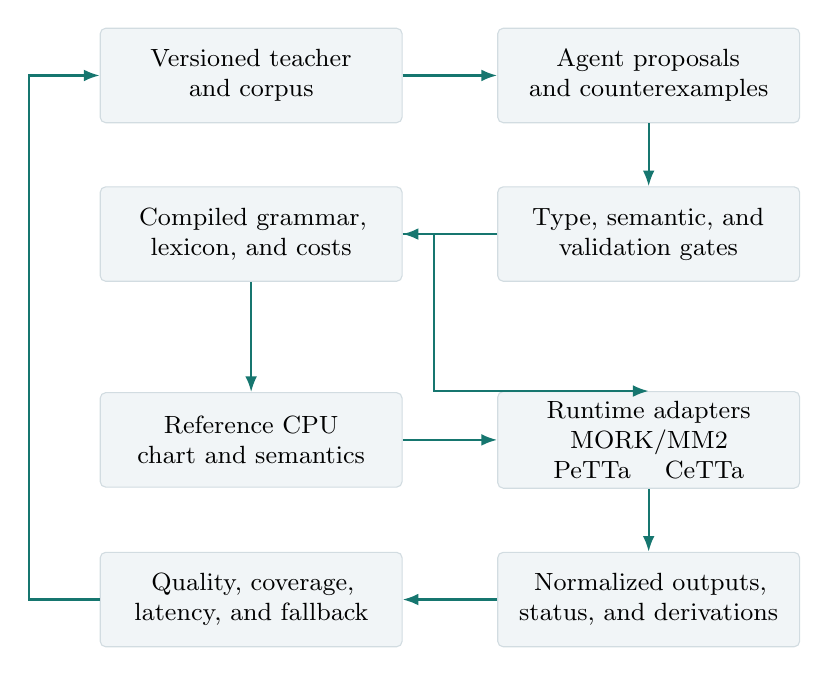
\begin{tikzpicture}[
  box/.style={draw=linegray,fill=pale,rounded corners=2pt,
    align=center,text width=36mm,minimum height=12mm,font=\small},
  arr/.style={-{Latex[length=2mm]},thick,draw=teal},
  node distance=8mm and 12mm]
\node[box] (teacher) {Versioned teacher\\and corpus};
\node[box,right=of teacher] (agents) {Agent proposals\\and counterexamples};
\node[box,below=of agents] (checks) {Type, semantic, and\\validation gates};
\node[box,left=of checks] (bundle) {Compiled grammar,\\lexicon, and costs};
\node[box,below=14mm of bundle] (ref) {Reference CPU\\chart and semantics};
\node[box,right=of ref] (mork) {Runtime adapters\\MORK/MM2\\PeTTa \quad CeTTa};
\node[box,below=of mork] (out) {Normalized outputs,\\status, and derivations};
\node[box,left=of out] (eval) {Quality, coverage,\\latency, and fallback};
\draw[arr] (teacher)--(agents);
\draw[arr] (agents)--(checks);
\draw[arr] (checks)--(bundle);
\draw[arr] (bundle)--(ref);
\draw[arr] (bundle.east) -- ++(4mm,0) |- (mork.north);
\draw[arr] (ref)--(mork);
\draw[arr] (mork)--(out);
\draw[arr] (out)--(eval);
\draw[arr] (eval.west) -- ++(-9mm,0) |- (teacher.west);
\end{tikzpicture}
\caption{Construction, execution, and measurement share one versioned
semantic contract. The reference implementation is retained as an oracle
for backend behavior; differential checks compare each runtime with the same reference.}
\end{figure}

\subsection{The immutable bundle}
A release bundle identifies the teacher data snapshot, ontology, grammar,
lexicon, category inventory, normalizer, ranker, compiler, common parser IR,
backend configuration manifests, and test manifest. The bundle has a content digest. Outputs record that digest,
the normalized input and context identifiers, parser configuration, and the
derivation or derivation references used.

Lexical records contain a lemma or expression, sense identifier, surface-form
or morphology reference, category template, semantic-template reference,
typed parameters, licensing conditions, source, and revision. An idiom is a
lexically anchored construction and belongs in this inventory unless a report
explicitly counts it separately. Inflected forms normally point to shared
records rather than duplicating semantic programs.

The compiler validates templates and creates concrete category IDs, permitted
transition IDs, lexical indexes, semantic-recipe IDs, and cost tables.
Compilation must reject unresolved features, unbound semantic variables,
unlicensed constructors, and illegal recursion. Finite domains are not a
license to instantiate their entire Cartesian product: only realizable,
licensed combinations should become runtime records.

\subsection{Output and error contract}
Every parse request reports two separate axes. Construction status is
\code{complete}, \code{truncated}, \code{no\_parse}, or \code{error}.
The acceptance decision is \code{accepted}, \code{ambiguous}, or
\code{abstain}. A complete forest can still be ambiguous; a truncated search
can still contain a candidate. Resource exhaustion is never reported as
proof that no grammatical analysis exists.

An accepted result contains a normalized interpretation, provenance, and an
acceptance decision under the declared calibration policy. An ambiguous result
contains a finite candidate set or a permitted unresolved structure.
Unsupported distinctions have named diagnostics. Fallback, if enabled, adds
the teacher output and its own provenance. It does not retroactively count as
successful symbolic coverage. The parser should not manufacture a complete
meaning by silently deleting unsupported material.

\subsection{What may influence packing and scoring}
Every field inspected by future rule legality or compositional cost must
appear in the chart interface. Examples include agreement, clause form,
normal-form history flags, and any declared semantic class used to license
a construction. Features used only after complete interpretation can remain
in semantic recipes and be handled by a separate reranker.

This restriction is central to the architecture. It prevents a later rule
from distinguishing two alternatives that the parser has already merged as
interchangeable. If a new selection feature needs the exact lexical head,
scope state, or discourse referent, the implementation must either refine the
interface and reconsider its complexity or defer that feature until after
candidate generation.

\section{The restricted CCG calculus}\label{sec:calculus}

\subsection{Finite categories and features}
Let \(\mathcal C\) be a finite inventory of fully specified categories. Atomic
categories include \(\NC\), \(\NP\), \(\SF\), \(\SB\), and \(\ST\), with
explicitly declared finite feature domains. The authoring language may use
feature variables and slash constructors, but the compiler produces licensed
concrete categories or an equivalently bounded matching representation.
Every category produced at runtime must belong to \(\mathcal C\).

A finite number of combinator schemas and a finite initial lexicon do not
alone establish this property. Unrestricted composition can create
increasingly complex categories. The compiler therefore enforces depth and
feature bounds and a finite admitted transition inventory. The language
covered by a release is the language of that admitted inventory, not all
derivations that an unrestricted CCG might license.

Syntactic feature metavariables, semantic lambda variables, logical bound
variables, runtime pattern variables, and persistent entity identifiers have
different namespaces. In particular, a runtime \code{\$x} pattern variable
must not accidentally become the implementation of a logical quantifier.

\subsection{Four binary combinators}
For adjacent nonempty spans, the initial calculus admits:
\begin{align}
 \mathrm{FA}:&\quad (X/Y,f)\ (Y,a)
       \Longrightarrow (X,f(a)), \label{eq:fa}\\
 \mathrm{BA}:&\quad (Y,a)\ (X\backslash Y,f)
       \Longrightarrow (X,f(a)),\\
 \mathrm{FC}:&\quad (X/Y,f)\ (Y/Z,g)
       \Longrightarrow (X/Z,\lambda z.\,f(g(z))),\\
 \mathrm{BC}:&\quad (Y\backslash Z,g)\ (X\backslash Y,f)
       \Longrightarrow (X\backslash Z,\lambda z.\,f(g(z))).
       \label{eq:bc}
\end{align}
FC and BC are degree-one harmonic composition. The backward rule's order
matters: the semantic function of the right constituent is the outer function.
There is no crossed composition, substitution combinator, or unbounded
generalized composition in this initial kernel.

Bounded composition has a substantive complexity motivation: Schiffer,
Kuhlmann, and Satta identify composition degree as the source of an
exponential factor in the grammar-size-sensitive parsing analysis they study
\cite{boundedccg}. Our simpler fixed-inventory chart bound is stated
separately in Section~\ref{sec:theory}. It does not follow merely from choosing
the name CCG.

\subsection{Licensed type raising and unary transitions}
For an explicitly listed target \(T\), possible type-raising variants are
\begin{align}
  \NP:q&\Longrightarrow T/(T\backslash\NP):\lambda f.\,f(q),\\
  \NP:q&\Longrightarrow T\backslash(T/\NP):\lambda f.\,f(q).
\end{align}
The conservative initial target is \(T=\SF\). Precompiled lexical variants
only raise the entries for which they are generated. Raising a compound noun
phrase such as \emph{every researcher} requires a licensed same-span unary
transition or an equivalent construction-specific macro. These are different
coverage decisions and must be recorded in the grammar manifest.

If unary transitions are admitted, their concrete transition graph is acyclic
and processed in a compiler-supplied topological order. No reverse conversion
may create a cycle. A type-raising operation is not a general invitation to
invent categories at runtime.

\subsection{Derivational normal forms}
Different CCG derivations may have beta-equivalent semantic construction
programs. Normal-form restrictions can reduce this redundancy
\cite{eisner}. For the first reference parser, preserve all licensed
derivations in the packed forest. Add restrictions only after demonstrating
that each equivalence class of interest retains a representative for the
actual finite grammar.

Store any restriction-relevant history in the chart interface. A rule that
depends on whether a constituent was formed by composition cannot safely
operate on a key that has discarded that history. Removing redundant
derivations can change Viterbi rankings when equivalent bracketings have
different costs, and changes probability mass if a later model sums over
derivations. Preserving semantics therefore does not by itself preserve the
selected output or probabilistic model; those are separate gates.

\section{Typed compositional semantics}\label{sec:semantics}

\subsection{Construction programs and logical representations}
Distinguish three objects: a syntactic derivation, its typed semantic
construction program, and a model-theoretic interpretation of the logical
representation it constructs. Parsing evaluates the construction program to produce a logical
representation, which then admits a model-theoretic interpretation. It does
not evaluate the truth of the input sentence.

Use base types \(\E\) for entity references, \(\V\) for event references,
\(\Prop\) for symbolic proposition representations, and \(\Int\) for
intensional-content representations. Define
\begin{equation}
 R=\E\to\Prop,\quad
 \Q=R\to\Prop,\quad
 \KK=\V\to\Prop,\quad
 \HH=\KK\to\Prop .
 \label{eq:types}
\end{equation}
The category interpretation is
\begin{align}
 \tau(\NC)&=R,&
 \tau(\NP)&=\Q,&
 \tau(\mathsf S_m)&=\HH,\\
 \tau(X/Y)&=\tau(Y)\to\tau(X),&
 \tau(X\backslash Y)&=\tau(Y)\to\tau(X).
\end{align}
Consequently \(\tau(\mathsf S_m\backslash\NP)=\VP=\Q\to\HH\), and a
transitive verb has type \(\Q\to\Q\to\HH\).
Clause-form features retain their syntactic significance even when their
semantic types coincide.

\subsection{A checked semantic language}
The authoring representation has variables, constants, abstraction, and
application. A representative abstract syntax is:
\begin{lstlisting}
Term := Var(index) | Const(symbol)
      | Lam(argument_type, body) | App(function, argument)
Type := Entity | Event | Prop | Intension | Arrow(Type, Type)
\end{lstlisting}
Use de Bruijn indices or another fully specified hygienic representation in
the trusted core. Named variables can be an authoring convenience, but the
compiler resolves them and rejects free names. Templates contain no arbitrary
runtime evaluation, I/O, recursion, mutation, or calls into an unrestricted
MeTTa evaluator.

The signature includes typed lexical predicates and logical constructors:
\begin{align*}
 \mathsf{Researcher},\mathsf{Paper}&:\E\to\Prop,\\
 \mathsf{Review},\mathsf{Leave},\mathsf{Past},\mathsf{Quick}&:\V\to\Prop,\\
 \mathsf{Agent},\mathsf{Theme},\mathsf{Recipient}&:\V\to\E\to\Prop,\\
 \SAnd,\mathsf{Implies}&:\Prop\to\Prop\to\Prop,\\
 \Not&:\Prop\to\Prop,\\
 \mathsf{ForallE},\mathsf{ExistsE}&:(\E\to\Prop)\to\Prop,\\
 \mathsf{ExistsV}&:(\V\to\Prop)\to\Prop,\\
 \Bx&:\Prop\to\Int,\qquad
 \mathsf{Content}:\V\to\Int\to\Prop .
\end{align*}
Constants for truth, falsity, and typed equality or inequality can be added
explicitly. The final formula representation uses fixed-arity nodes and
logical binders. For example,
\(\mathsf{ForallE}(\lambda x.\phi)\) lowers to an object-language
\(\forall x{:}\E.\phi\) node. Lambda abstraction used to build a formula and
logical quantification inside that formula are distinct operations.

The initial resource discipline limits template size and higher-order
argument duplication. Treat functional inputs such as noun-phrase
continuations, verb phrases, and event continuations affinely where possible:
each is consumed at most once by a template. Reusing an entity reference in
several roles is allowed. Affineness is a useful engineering restriction;
it is not, by itself, a complete runtime bound for every extension.

\subsection{Uniform noun phrases}
All noun phrases have type \(\Q\). A proper name is lifted:
\begin{equation}
   \Unit(a)=\lambda k^{R}.\,k(a).
\end{equation}
Determiners of category \(\NP/\NC\) include
\begin{align}
 \mathit{every}
   &=\lambda r^{R}.\lambda k^{R}.
       \forall x{:}\E\,\bigl(r(x)\Rightarrow k(x)\bigr),\\
 \mathit{a}
   &=\lambda r^{R}.\lambda k^{R}.
       \exists x{:}\E\,\bigl(r(x)\land k(x)\bigr).
\end{align}
Thus \(\mathit{every}(\mathsf{Researcher})\) and
\(\Unit(\mathsf{alice})\) have the same semantic interface. A quantified noun
phrase cannot accidentally be passed to a role that expects an entity.
The grammar must open it through its continuation.

\subsection{Event continuations and root closure}
A clause carries a continuation \(k:\V\to\Prop\) for its relevant event:
\begin{equation}
  \Close(h)=h(\lambda e^{\V}.\top):\Prop.
  \label{eq:close}
\end{equation}
An intransitive example is
\begin{equation}
 \mathit{leave}
 =\lambda q^{\Q}.\lambda k^{\KK}.
   q\!\left(\lambda x^{\E}.
    \exists e{:}\V[
      \mathsf{Leave}(e)\land\mathsf{Agent}(e,x)\land k(e)]\right).
 \label{eq:leave}
\end{equation}
The event witness is introduced inside the noun phrase's scope. A value of
type \(\HH\) is not a globally existing event object. In a negated clause,
the existential and the continuation may both occur under negation.

For a transitive verb, define the illustrative frame
\[
 F(e,s,o)=
 \mathsf{Review}(e)\land\mathsf{Agent}(e,s)\land
 \mathsf{Theme}(e,o)\land\mathsf{Past}(e).
\]
Two explicitly licensed local scope templates are
\begin{align}
 \mathit{review}_{S}
 &=\lambda q_o^{\Q}.\lambda q_s^{\Q}.\lambda k^{\KK}.
 q_s\!\left(\lambda s.
 q_o\!\left(\lambda o.\exists e{:}\V[F(e,s,o)\land k(e)]\right)\right),
 \label{eq:tvsubj}\\
 \mathit{review}_{O}
 &=\lambda q_o^{\Q}.\lambda q_s^{\Q}.\lambda k^{\KK}.
 q_o\!\left(\lambda o.
 q_s\!\left(\lambda s.\exists e{:}\V[F(e,s,o)\land k(e)]\right)\right).
 \label{eq:tvobj}
\end{align}
The syntactic argument order is object, subject; the semantic quantifier
nesting is selected by the template. With names, these alternatives reduce
to the same reading. With quantifiers, they can differ.

Root closure of \emph{Every researcher reviewed a paper} gives, respectively,
\begin{align}
 &\forall s\bigl(\mathsf{Researcher}(s)\Rightarrow
       \exists o[\mathsf{Paper}(o)\land\exists e\,F(e,s,o)]\bigr),
       \label{eq:scopeone}\\
 &\exists o\bigl(\mathsf{Paper}(o)\land
       \forall s[\mathsf{Researcher}(s)\Rightarrow
                      \exists e\,F(e,s,o)]\bigr).
       \label{eq:scopetwo}
\end{align}
In a model with two researchers who reviewed different papers and no common
paper, the first is true and the second false. These alternatives must not be
merged by canonicalization.

This is a local scope mechanism. Composition and type raising with fixed
semantics can merely rebracket the same meaning; they do not automatically
generate every scope reading. Additional quantifiers, scope islands, modals,
and negative polarity require specified templates or a richer scope
representation.

\subsection{Modifiers constrain the correct event}
For a postverbal manner modifier with category
\((\SF\backslash\NP)\backslash(\SF\backslash\NP)\), use
\begin{equation}
 \mathit{quickly}
 =\lambda vp^{\VP}.\lambda q^{\Q}.\lambda k^{\KK}.
       vp(q)(\lambda e.\mathsf{Quick}(e)\land k(e)).
 \label{eq:quick}
\end{equation}
Emit the same semantic template at each explicitly licensed clause form
\(m\), with category
\((\mathsf S_m\backslash\NP)\backslash(\mathsf S_m\backslash\NP)\).
This places \(\mathsf{Quick}(e)\) inside the existential binder for the same
event supplied by the verb. If Alice reviewed Bob slowly while an unrelated
event was quick, the unrelated event cannot satisfy this modifier.

The continuation has a declared head-event interpretation. It does not give
every modifier access to every embedded event. A modifier of an embedded
leaving event must attach to the embedded verb phrase before closure; a
modifier of a promise event attaches to the matrix clause.

\subsection{Negation preserves quantifier and event scope}
One subject-wide VP-negation template is
\begin{equation}
 \mathit{NegVP}
 =\lambda vp^{\VP}.\lambda q^{\Q}.\lambda k^{\KK}.
     q\!\left(\lambda s.\neg\bigl(vp(\Unit(s))(k)\bigr)\right).
 \label{eq:negvp}
\end{equation}
Its category can be
\((\SB\backslash\NP)/(\SB\backslash\NP)\) for a selected auxiliary analysis.
Tense and auxiliary licensing are separate grammatical specifications.
With a name and a leaving VP, root closure yields
\[
 \neg\exists e\,
   [\mathsf{Leave}(e)\land\mathsf{Agent}(e,\mathsf{alice})].
\]
Moving the event existential outside negation produces a different formula.
The original can be true when there is no leaving event. An implementation
that always allocates an asserted head event before processing negation is
therefore incorrect.

The placement of \(q\) in Equation~\eqref{eq:negvp} gives an every--not
reading for a universal subject. A not--every reading needs an explicitly
different construction:
\[
  \forall x(R(x)\Rightarrow\neg L(x))
  \quad\hbox{versus}\quad
  \neg\forall x(R(x)\Rightarrow L(x)).
\]
A model in which some but not all researchers leave separates them. The
grammar must license the intended alternatives and selection policy rather
than let an arbitrary rewrite decide.

\subsection{Control, reference sharing, and intensional contents}
Consider a selected recipient-taking lexical frame with category
\[
  ((\SF\backslash\NP)/(\ST\backslash\NP))/\NP .
\]
Its syntactic arguments are the recipient NP, embedded infinitival VP, and
subject NP, in that order. The event continuation is a further semantic
parameter, not another syntactic constituent. Let \(C(s,o)\) select the controller:
\(C(s,o)=s\) for subject control and \(C(s,o)=o\) for object control.
The selector is a compile-time choice between these two projections. A template is
\begin{align}
 &\mathit{Control}_{K,C}
   =\lambda q_o^{\Q}.\lambda vp_c^{\VP}.\lambda q_s^{\Q}.\lambda k^{\KK}.
      q_s\!\left(\lambda s.\,q_o\!\left(\lambda o.
      \exists e\,[\,K(e)\land\mathsf{Agent}(e,s)
          \land\mathsf{Recipient}(e,o)\right.\right.\nonumber\\[-1mm]
 &\hspace{24mm}\left.\left.
       {}\land\mathsf{Past}(e)
       \land\mathsf{Content}\!\left(e,
          \Bx\!\left(\Close(vp_c(\Unit(C(s,o))))\right)\right)
       \land k(e)\,]\right)\right).
 \label{eq:control}
\end{align}
Here \(K\) is a declared event predicate such as \(\mathsf{Promise}\) or
\(\mathsf{Persuade}\). The frame is illustrative; a production ontology may
assign finer role names and additional lexical commitments.

For \emph{Alice promised Bob to leave}, the boxed content contains Alice as
the agent of leaving. For \emph{Alice persuaded Bob to leave}, it contains
Bob. In these affirmative proper-name examples, the matrix event is asserted
while the embedded leaving proposition remains inside content. Neither template includes a
rule asserting that the leaving occurred.

With \emph{Every researcher promised Bob to leave}, the subject quantifier
is opened once. The resulting entity reference \(s\) appears both as matrix
Agent and inside the boxed proposition. Reusing the original generalized
quantifier in the embedded clause would introduce an independent
quantification instead of retaining the same individual reference. Sharing a bound reference is the required operation.

\subsection{A semantic foundation for Box}
\(\Bx\) receives a proposition representation, not an eagerly evaluated
Boolean. One possible foundation interprets its argument intensionally:
\[
  \sem{\Bx(\phi)}^\rho
     =\bigl(w'\mapsto\sem{\phi}_{w',\rho}\bigr),
\]
For this illustrative convention, entity and event domains are fixed, the
assignment \(\rho\) to outer references is retained across worlds, and
predicates may vary with the world. \(\mathsf{Content}\) is a relation between the matrix
event and such an intension. There is no axiom
\(\mathsf{Content}(e,\Bx(\phi))\Rightarrow\phi\).

This foundation is optional and is not an implemented modal reasoner.
If the target requires hyperintensional or verbatim content, even some
logically equivalent propositions must remain distinct. The normalization
contract must state which transformations are admissible inside each
content constructor. The reference checker only tests that content is
non-eager and non-asserting.

\subsection{Event identity and the limits of the H interface}
Distinct binders introduce distinct variable positions, not necessarily
different denotations. The formula
\(\exists e_1\exists e_2[L(e_1)\land L(e_2)]\) permits \(e_1=e_2\).
A reading of \emph{twice} that requires two occurrences must add
\(e_1\ne e_2\), an event-cardinality construction, or another explicit
distinctness condition.

The single-event continuation \(\HH\) is intentionally limited. Naively
defining clause coordination by applying the same continuation to both clauses
duplicates a higher-order argument and exposes two events through an
interface designed for one. Coordination needs an event-group interface,
separate exposed ports, or a declared closure policy. Stative predication
likewise requires a decision about eventualities or a separate proposition
interface. These extensions are work-plan tasks, not capabilities conferred
automatically by the current types.

\subsection{Storage does not assert represented facts}
If a formula is stored in Atomspace or MORK, its internal
\(\mathsf{Agent}\), \(\mathsf{Leave}\), and other nodes must retain parse,
scope, and binder membership. A represented predicate under \(\Not\) or
\(\Bx\) must not become an independently asserted fact in the global
reasoning space. Use a tagged formula graph or scoped node records, and a
separate API for promoting justified assertions. This remains necessary even
when all representations happen to be S-expressions.

\section{SENF as an executable normalization contract}\label{sec:normalization}

\subsection{The exact layer}
Define an explicit equational theory \(E_0\) for the first release.
At the construction-program level it includes capture-avoiding beta
equivalence and alpha-equivalence. At the formula level it includes a small
set of structural identities, initially associativity and commutativity of
conjunction and removal of its truth unit. It preserves predicate names, role
labels, argument order, binder order, event identity constraints, negation,
and content boundaries.

The full output pipeline has fixed phases. In the laws below, \(\NF\)
denotes canonicalization of well-scoped formula syntax after clause closure
and lowering; beta reduction of construction programs is a separate typed
stage.
\begin{enumerate}
  \item Validate the category/semantic type and all bound-variable references.
  \item Materialize one selected semantic recipe with hygienic substitution.
  \item Apply required root closure, then beta-normalize the construction
  program. Logical quantifiers remain constructors, not evaluated loops.
  \item Lower quantifier constructors to explicit typed binder nodes.
  Preserve the binding environment of boxed contents.
  \item Recursively normalize children under the policy of each enclosing
  constructor. Where conjunction identities are licensed, flatten directly
  nested conjunctions, remove \(\top\), and sort the remaining children by
  a canonical structural order. Rebuild a right-associated binary
  \(\SAnd\); a singleton becomes its child and an empty list becomes
  \(\top\).
  \item Produce deterministic serialization, structural sharing where
  binding-safe, and a transformation trace.
\end{enumerate}
Construction-time beta reduction computes a boxed payload even when that
payload is opaque to later logical rewrites. New content constructors default
to opacity. The initial intensional \(\Bx\) profile explicitly permits
binding hygiene and the listed conjunction identities within its payload;
those identities hold at every world under the illustrative interpretation.
A hyperintensional profile uses a stricter whitelist, and verbatim quotation
requires a separate text-preserving constructor. The chosen profile is part
of the schema version.

Do not flatten across a quantifier, negation, or content boundary. Retain
repeated children unless an additional identity has explicitly been adopted;
conjunction normalization does not imply event merging.

Canonical ordering must compare meaning-bearing syntax rather than
allocation IDs. Hashes may accelerate comparison, but collisions are checked
against the full structure. A shared subtree containing bound references is
safe only with its binding interface or environment; globally identifying all
occurrences of \code{Var(0)} as one entity would be incorrect.

\subsection{What equality of normal forms means}
For the declared interpretation class and congruence policy, require:
\begin{align}
 \NF(\NF(t))&=\NF(t), \label{eq:idempotence}\\
 \sem{\NF(t)}&=\sem{t}, \label{eq:nfsound}\\
 \NF(t)=\NF(u)&\Longrightarrow \sem{t}=\sem{u}. \label{eq:nfeq}
\end{align}
The equality in Equation~\eqref{eq:nfsound} includes the target's treatment of
boxed contents. Under the possible-world interpretation, a rewrite inside a
box must preserve truth at every relevant world and assignment. Under a
hyperintensional policy, only the explicitly permitted representational
identities may be used there. A rewrite justified only by facts true in the
actual world cannot automatically be applied inside a belief or promise
content.

The reverse implication in Equation~\eqref{eq:nfeq} is not promised. For
example, independent existential quantifiers might be logically
interchangeable, but this initial normalizer preserves their order. Leaving
such formulas distinct is a known limitation, not a reason to introduce an
unbounded equivalence prover into parsing.

Likewise, deterministic idempotent normalization is not automatically a
proof that an arbitrary rewrite system is confluent or that its output is
globally smallest. Confluence requires analysis of the actual rewrite
relation; global minimality requires a specified representation language and
cost. The implementation initially claims a canonical representation under
its selected structural theory and a deterministic algorithm, with no
universal graph-minimization claim.

\subsection{Early normalization and compositional compatibility}
For partial results, let \(N\) denote a family of type-preserving normalizers;
root closure is excluded until a declared clause boundary. Normalization
during chart construction is safe only when it is compatible
with every later semantic constructor \(F\):
\begin{equation}
 N(F(t_1,\ldots,t_r))
  =N(F(N(t_1),\ldots,N(t_r))).
 \label{eq:congruence}
\end{equation}
This equation is an obligation for a proposed optimization, not a property
of every plausible simplification. Initial deployment can avoid the issue by
normalizing only selected complete interpretations, while storing pure
semantic recipes in the forest. Later, safe local canonicalization can reduce
duplication if Equation~\eqref{eq:congruence} is established for it.

\subsection{Learned consolidation as a separate operation}
Let \(N_0\) denote exact normalization and \(A_{\theta,c}\) a learned
consolidation or abstraction under policy \(\theta\) and context \(c\).
A result can contain both:
\[
  \bigl(N_0(t),\ A_{\theta,c}(N_0(t)),\ \text{links and provenance}\bigr).
\]
Useful examples include a macro for a recurring semantic subgraph, a
domain-specific synonym mapping, or a query-specific projection to event
participants. A macro with a checked inverse expansion can be lossless.
A role projection generally is not.

For a query family \(\mathcal Q\), a useful abstraction criterion is:
\[
   q(t)=\widetilde q(A_{\theta,c}(t))
   \quad\text{for all declared }q\in\mathcal Q,
\]
with an explicit interpretation \(\widetilde q\) on the abstract graph.
This expresses adequacy for named uses without asserting full semantic
equivalence. The criterion may be proved for simple projections and tested
empirically for learned ones. Confidence scores do not replace a missing
proof where exact equivalence is required.

Fuzzy similarity is not necessarily transitive. If \(a\) is similar to \(b\)
and \(b\) to \(c\), collapsing all three into one equivalence class can erase
a distinction between \(a\) and \(c\). Store approximate relations or
policy-specific abstractions without using them as the global equality
relation for exact chart packing.

\subsection{Enrichment and causal annotations}
Background PLN inference may add consequences, hypotheses, or probabilistic
links. Represent each addition with its premises, inference method, knowledge
version, confidence interpretation, and scope. Preserve the sentence's
asserted content separately. A textual \emph{because} relation can represent
the speaker's causal claim; it is not, by itself, a validated causal model.

The supplied FUSE-NF manuscript proposes graph-transformer use as a further
application \cite{senf}. The present parser can export graphs for that
purpose, but neither a transformer nor causal discovery is needed to
establish the symbolic parsing experiment. Keeping the interfaces separate
also makes it possible to compare exact semantics, abstractions, and
enrichment independently.

\addtocontents{toc}{\protect\newpage}
\section{Conditional correctness and complexity}\label{sec:theory}

The statements below are relative guarantees for a specified finite grammar
and semantic language. They do not prove that its lexicon describes English
correctly, that it covers the teacher's outputs, or that its selected reading
is the intended one.

\begin{assumption}[Checked lexical and construction signatures]
Every lexical entry of category \(C\) supplies a closed construction term
of type \(\tau(C)\). Each licensed unary transformation has its declared
function type. Logical constructors and lexical predicates have fixed types.
Binding is hygienic, and no effectful or recursive evaluator is hidden in a
semantic constant.
\end{assumption}

\begin{proposition}[Type preservation of derivation]\label{prop:typing}
Under the checked-signature assumption, every derivation of category \(C\)
using the four binary combinators and licensed unary transformations
constructs a term of type \(\tau(C)\).
\end{proposition}
\begin{proof}
Induct on the derivation. Lexical leaves satisfy the assumption. In FA,
\(\tau(X/Y)=\tau(Y)\to\tau(X)\), so applying the left meaning to the
right meaning has type \(\tau(X)\). BA has the same function typing with
the syntactic children reversed. In FC, \(g:\tau(Z)\to\tau(Y)\) and
\(f:\tau(Y)\to\tau(X)\), so \(\lambda z.f(g(z))\) has type
\(\tau(Z)\to\tau(X)\). BC uses the same composition in the declared
backward order. A checked unary transformation preserves its declared
source-to-target relation. These cases exhaust the derivation.
\end{proof}

\begin{proposition}[Well-scoped closure]
A closed root term of type \(\HH\) yields a closed proposition under
\(\Close\). In Equation~\eqref{eq:control}, closing the embedded clause and
boxing it preserves the reference to the chosen controller without
introducing another controller quantifier.
\end{proposition}
\begin{proof}
\(\lambda e.\top\) has type \(\KK\), so applying a closed
\(\HH=\KK\to\Prop\) term to it produces a closed \(\Prop\) term.
Inside control, \(\Unit(C(s,o)):\Q\), hence
\(vp_c(\Unit(C(s,o))):\HH\), its closure has type \(\Prop\), and its
box has type \(\Int\). The references \(s,o\) are bound by the enclosing
continuations. Hygienic substitution preserves those references; no new
application of \(q_s\) or \(q_o\) is introduced by \(\Unit\).
\end{proof}

\begin{proposition}[Restricted normalization]
For well-typed pure construction terms, capture-avoiding beta reduction
preserves type and construction meaning. After lowering, the recursive
conjunction canonicalizer is terminating and idempotent, and preserves the
selected interpretation when its identities are congruences at every
constructor where they are applied.
\end{proposition}
\begin{proof}
Type preservation of beta reduction follows from the typed substitution
lemma: substituting a term of the binder's type preserves the body's type.
The pure simply typed lambda core has normalization \cite{tapl}; no recursive constant
or additional nonterminating rewrite is admitted. For the formula phase,
recursive calls traverse finite children. Flattening removes nested
conjunction structure, truth-unit removal deletes nodes, and sorting is a
finite deterministic operation. A second pass finds normalized children and
the same flattened, sorted list. The identities preserve conjunction under
the declared interpretation; the congruence condition permits substitution
into surrounding constructors. Composition of these sound phases gives the
claim.
\end{proof}

This proof does not bound the size or time of beta normalization for arbitrary
higher-order terms. A production compiler also enforces resource restrictions
on templates and monitors materialized output size. The finite chart theorem
below concerns the packed derivation structure, not enumeration of every
logical form.

\begin{assumption}[Finite acyclic chart fragment]\label{assump:finite}
For a fixed grammar bundle, the chart has \(C\) possible category/interface/
control signatures per span. Binary rules combine adjacent nonempty
subspans and belong to a finite compiled transition inventory \(\mathcal B\).
Unary transitions belong to a finite acyclic inventory \(\mathcal U\).
Each emitted edge has a finite immutable recipe and a canonical identity.
\end{assumption}

\begin{proposition}[Finite chart and a restricted cubic bound]
For \(n\) tokens and \(\ell\) lexical edges, an exhaustive span-ordered
construction under Assumption~\ref{assump:finite} terminates. It has
\(O(n^2 C)\) nodes and at most
\[
 O\!\left(n^3|\mathcal B|+n^2|\mathcal U|+\ell\right)
\]
edges. With bounded-cost indexed operations, this expression also bounds
the elementary construction work up to implementation-dependent constants.
\end{proposition}
\begin{proof}
There are \(n(n+1)/2\) nonempty spans and at most \(C\) signatures for
each. There are \(O(n^3)\) triples \(i<k<j\), each admitting at most the
finite inventory of binary transition instances. Unary edges are bounded
per span by \(|\mathcal U|\). Span width strictly increases across binary
dependencies, and unary dependencies follow a finite topological order.
Canonical insertion prevents duplicate jobs from creating new identities
indefinitely. Lexical edges contribute \(\ell\).
\end{proof}

The constant \(C\) must actually be fixed independently of sentence length
for the usual cubic interpretation. Adding an arbitrary lexical-head token
position introduces an additional \(O(n)\) state factor. Naive joins over
both child head positions can then take \(O(n^5)\). Similar caveats apply to
unbounded context IDs or semantic values in chart keys. These extensions may
be worthwhile, but their complexity must be measured and analyzed explicitly.

\begin{assumption}[Complete observable interface]\label{assump:interface}
Every future legality test and local cost depends only on the input/context,
rule identity, and declared child chart signatures. Semantic recipes are pure
and act on selected child meanings without a hidden applicability test.
Alternative incoming edges remain represented.
\end{assumption}

\begin{proposition}[Packing preserves licensed derivations]\label{prop:packing}
Under Assumptions~\ref{assump:finite} and \ref{assump:interface}, replacing
explicit subderivations with one node per chart key and its alternative
incoming edges preserves the derivations and constructed meanings of the
declared grammar.
\end{proposition}
\begin{proof}
Induct in the acyclic chart order. Every explicit lexical derivation has its
lexical edge. For an explicit binary or unary derivation, its child
derivations are represented by induction. The interface assumption ensures
the same rule remains licensed for their keys, and the associated edge
records the same construction recipe. Conversely, unpacking an edge chooses
represented child derivations to which that source rule applies and
constructs exactly its meaning. Keeping alternative edges avoids identifying
their resulting values. This gives both directions.
\end{proof}

For a counterexample to an incomplete key, suppose a later rule admits only
animate subjects, but animate and inanimate alternatives share a key that
omits the relevant sort. Accepting the rule for that key admits illegal
derivations; rejecting it loses legal ones. The compiler must refine the
interface or postpone the decision.

\begin{proposition}[Exact best-derivation decoding]\label{prop:viterbi}
If derivation cost is the sum of local edge costs and the interface
assumption holds, bottom-up minimum-cost evaluation on the acyclic forest
returns the least-cost licensed derivation. A fixed structural tie policy
makes the selected derivation deterministic.
\end{proposition}
\begin{proof}
For each node, an admissible derivation consists of an incoming edge and one
derivation for each child. Additivity and interface sufficiency make the
minimum for an edge its local cost plus the independently optimal child
costs. Taking the minimum over incoming edges and inducting in acyclic order
gives the result.
\end{proof}

This is a best-derivation result. If several derivations yield one normalized
meaning \(y\), its probability under a probabilistic model would involve
\[
  p(y\mid x)=\sum_{d:\,N(\sem d)=y}p(d\mid x).
\]
The most probable \(y\) need not be the meaning of the most probable single
derivation. The initial scalar costs are not asserted to be probabilities.

\begin{proposition}[Conditional backend correspondence]\label{prop:backend}
Suppose the compiler preserves lexical records, transition predicates,
recipes, and local costs; backend indexes are exact projections of canonical
records; every deduction is executed after its premises are complete;
and duplicate insertion preserves all distinct edge identities. Then the
backend constructs a forest isomorphic to the reference forest, up to
internal IDs, and selects the same normalized output under the same tie rule.
\end{proposition}
\begin{proof}
Induct over span width and the unary topological order. Corresponding lexical
inputs establish the base. Exact indexes and complete scheduling supply
precisely the premises for each source transition; compiler preservation
gives the same parent and recipe. Idempotence removes only duplicate
identities. Thus each phase yields corresponding node and edge sets.
Proposition~\ref{prop:viterbi} and shared semantic construction then give
matching selected outputs.
\end{proof}

The assumptions are implementation proof obligations. Differential testing
on exhaustive small grammars and adversarial inputs is the first practical
way to detect their violation; passing a finite suite is not a general formal
verification of the backend. Apply the proposition independently to
\(b\in\{\text{MORK/MM2},\text{PeTTa},\text{CeTTa}\}\); common MeTTa
notation does not establish any of its premises. For a different internal
representation, define and check its projection to the canonical logical
forest before claiming correspondence.

\section{Packed parsing, selection, and semantic extraction}\label{sec:chart}

\subsection{Chart nodes and forest edges}
For a fixed sentence, a chart node has key
\[
  K=(\mathit{sentence},i,j,\mathit{category},
                    \mathit{interface},\mathit{control}),
  \qquad 0\le i<j\le n.
\]
The category contains the grammatical features. The interface contains every
semantic distinction visible to later local guards and scores. The control
component records finite derivational history needed by licensed
normal-form restrictions. Fields may be combined into an interned signature,
but their meaning remains explicit.

Use separate identities for a packed state, a fully constructed semantic
value, and provenance. Representative records are:
\begin{lstlisting}
Node(node_id, sentence_id, i, j, category_id, interface_id, control_id)
Edge(edge_id, parent_id, rule_id, ordered_child_ids,
     recipe_id, local_cost)
LexEdge(edge_id, parent_id, lexical_entry_id, recipe_id, local_cost)
Source(edge_id, source_rule_id, source_revision, source_location)
\end{lstlisting}
An edge identity is its canonical structural tuple, including every local
choice that matters. Re-inserting that tuple is idempotent. Distinct
lexical senses or scope recipes remain distinct edges even when they have
the same parent. Allocation-order IDs must not determine semantic choices
or backend equality.

A node denotes a set of derivations. Attaching one materialized meaning to
the node would discard alternatives; attaching all their role facts to one
graph would combine incompatible meanings. Each selected derivation instead
chooses one incoming edge at each step and materializes its own scoped
semantic value.

\subsection{An exact reference algorithm}
Start with exhaustive construction for the finite admitted grammar:
\begin{lstlisting}
for width in 1 .. number_of_tokens:
    for each span [i, j) of this width:
        add every licensed lexical edge covering [i, j)
        for split in i+1 .. j-1:
            for each compatible pair of completed child states:
                add the licensed parent state and recipe edge
        apply permitted unary transitions in topological order
        mark this span complete

score the resulting acyclic forest
extract requested root derivations and construct their meanings
\end{lstlisting}
Multiword lexical entries occupy ordinary nonempty spans. Their lookup must
occur for each supported span before it is finalized. A multiword expression
and a compositional reading can coexist as alternatives.

The first implementation separates forest construction from scoring.
This makes missed deductions easier to distinguish from ranking errors and
avoids score-improvement races. Resource budgets are checked explicitly;
exceeding one produces \code{truncated}, even if a root candidate has already
been found.

\subsection{Weights and decoding}
Use an additive cost model:
\[
  \Cost(d)=\sum_{e\in d}c(e),\qquad
  V(v)=\min_{e:\,\operatorname{parent}(e)=v}
           \left(c(e)+\sum_{u\in\operatorname{children}(e)}V(u)\right).
\]
Lexical edges have no children. Fixed-point or integer costs simplify exact
cross-backend comparison. Overflow, infinity, and tie resolution have
defined behavior. An acyclic forest permits negative edge costs in principle,
but nonnegative costs can simplify later best-first search; the first
implementation should choose and document one convention.

Costs can depend on lexical choices, declared construction features,
fixed input context, and child interfaces. A sparse feature score can be
computed through scalar additions and table lookups. A feature that reads
a hidden complete child meaning violates the packing premise. Put it in a
declared interface or use it in an explicitly separate candidate reranker.

The cost itself is not a confidence estimate. Confidence or acceptance
probability is calibrated against an error definition on held-out data.
Possible predictors include score margins, lexical novelty, construction
support, competing normalized meanings, and resource-limit indicators.
They can be implemented as symbolic decision rules or scalar models.

\subsection{Materializing meanings and handling duplicate outputs}
Extract the best derivation first. Interpret its recipes in an immutable
typed AST or binding-safe DAG, close the required clauses, and normalize the
result. Cache values by a semantic recipe and a complete environment identity.
Do not reuse fresh binders across different instantiations by accident.

For multiple outputs, a lazy \(k\)-best derivation procedure can produce
candidates that are normalized and deduplicated. Many derivations may map to
one normalized output, so examining \(k\) derivations does not guarantee
\(k\) distinct meanings. The extraction budget and duplicate count belong
in the result.

On tiny grammars, enumerate all derivations and compare their meanings to
the packed representation. On larger inputs, the presence of an acceptable
teacher target among examined candidates establishes representability for
that example. Its absence in a bounded list does not prove that the full
forest lacks it. Reports should call this \emph{oracle-at-\(k\)} or another
explicitly bounded measure.

\subsection{Pruning is a subsequent, measured approximation}
Once exact construction is independently validated, add lexical pruning,
beam limits, agenda priorities, or bounded candidate extraction as separate
modes. For each, measure whether the teacher-compatible candidate is lost,
not merely whether some parse remains. Report speed and memory together
with the loss in oracle and selected-output quality.

If a global reranker selects from a bounded candidate list, the output is
optimal only within that list. A richer local interface may recover exact
dynamic programming at greater cost; this tradeoff should be studied rather
than hidden in implementation details.

\section{Compilation and comparative runtime execution}\label{sec:mork}

\subsection{One checked language and a common parser IR}
The authoring syntax can be MeTTa-shaped while remaining a deliberately
small DSL. A possible surface declaration is:
\begin{lstlisting}
; Illustrative authoring DSL; lowered by a checked compiler
(Lex reviewed
     (Fwd (Bwd (S finite) NP) NP)
     (Instantiate ReviewTransitive subject-wide)
     (Cost 10)
     (Source reviewed-transitive-v1))
\end{lstlisting}
This declaration becomes typed compiler data. Grammar parameters, source
IDs, morphology references, binding, and feature constraints are checked
before backend code is generated. The compiler emits a common IR containing
finite lexical records, category/interface IDs, transition tables, acyclic
unary order, typed semantic recipes, scalar costs, and provenance.

Reject a reachable category closure that exceeds its declared bound.
Do not silently truncate it and call the result equivalent compilation.
The same immutable IR and sentence lexicalization feed all three adapters.
Backend-specific code may change representation and execution strategy
while preserving the declared logical contract; it may not change the
grammar, cost tables, scope readings, or normalization profile.

\subsection{Adapter contract and configuration identity}
An adapter implements bundle loading, sentence initialization, phase
execution, completion detection, canonical forest export, and shutdown.
It also reports failures and resource exhaustion without converting them
into grammatical \code{no\_parse}. The initial common operations are:
\begin{enumerate}
  \item Insert or find a canonical ground chart node.
  \item Enumerate compatible neighboring nodes and transition records.
  \item Insert every distinct licensed hyperedge with its recipe and cost.
  \item Complete the required binary and unary deductions for a phase.
  \item Return a canonical view for reference comparison and extraction.
\end{enumerate}
These are interface obligations, not claims that every runtime supplies
identically named primitives. A verified host controller or helper is
permitted, but its work and transfer costs belong to that configuration.
Track A fixes the computational partition across its matched primary rows.
Adapter-specific representation conversion and marshalling may vary and are
measured. A helper that moves a logical operation from runtime to host
creates an additional configuration, unless the same partition change is
applied to every matched row. If a primary adapter cannot implement a required
runtime operation under that partition, its profile remains unsupported.

\begin{table}[htbp]
\small
\begin{tabularx}{\textwidth}{L{25mm}YY}
\toprule
Candidate & Primary configuration & Questions the adapter must resolve \\
\midrule
MORK/MM2 & Direct MM2 execution in a pinned MORK build. &
Consumed instructions, join completeness, phase barriers, and exact
index projections. \\
PeTTa & Pinned upstream PeTTa, SWI-Prolog, and its ordinary store. &
Compiled versus dynamic evaluation, load order, finite answer exhaustion,
duplicate proofs, and update visibility. \\
CeTTa & Pinned native C evaluator/store, explicit PeTTa dialect/profile. &
Completion versus interruption, inert data versus evaluated answers,
available primitives, and exact profile behavior. \\
\bottomrule
\end{tabularx}
\caption{The primary three-way comparison. All behavior is qualified by
executable probes. Optional bridges form additional configurations.}
\end{table}

Every run records a configuration tuple:
\[
 b=(\text{repository/commit},\text{build},\text{dependencies},
     \text{dialect/profile},\text{evaluator/store},\text{host split}).
\]
PeTTa with MORK spaces and CeTTa's MORK/MM2 bridge are separately labeled
hybrids \cite{petta,cetta}. A CeTTa run that delegates its chart work to
MORK cannot establish the speed of its native C execution. The primary native CeTTa chart configuration excludes Prolog execution;
Prolog-assisted configurations are separate rows. Where foreign callbacks
perform required work, record that delegation and its cost.
The pure symbolic parser uses no neural or matrix-based computation,
irrespective of unused facilities available elsewhere in a runtime.

\subsection{Capability probes before performance claims}
M10 produces a matrix of \emph{verified native}, \emph{verified with a
declared helper}, \emph{unsupported}, or \emph{unverified} operations for
each pinned build. A failed build or unrun probe is missing evidence, not
proof of unsupported semantics. Conformance requires every mandatory finite
qualification case to finish and agree with the reference; agreement only on
a self-selected subset of completed cases is insufficient.
Probe repeated-variable equality, variable freshening, ground-term
round trips, nested matching, duplicate insertion, distinct-edge retention,
mutation visibility, complete finite enumeration, empty results, completion
signals, interruption, integer cost behavior, and deterministic tie inputs.
Include resource cleanup and isolation between sentences.

For PeTTa, exercise declaration/load order and compiled versus dynamic
calls \cite{pettacompiler}. For CeTTa, distinguish a returned inert
expression, logical failure, a completed value stream, and interruption
under the chosen profile \cite{cettaledger}. For MORK, explicitly test
consumption of a no-match \code{exec} and the chosen barrier mechanism.
No adapter may count an unevaluated operation as a successfully computed
answer. An unsupported primitive remains a visible capability result;
the compiler must reject its use or select an explicitly reported helper.

\subsection{Logical indexes and physical representations}
Representative logical indexes are:
\begin{lstlisting}
(ByStart sentence category start end interface control node)
(ByEnd   sentence category end start interface control node)
(CombineLeft  grammar left_category right_category result rule)
(CombineRight grammar right_category left_category result rule)
\end{lstlisting}
Canonical node and edge records are authoritative; indexes are projections.
A left constituent ending at \(k\) selects permitted transitions, then
right constituents starting at \(k\) with compatible category and interface.

For MORK, placing grounded fields before unbound suffixes follows the
documented indexing considerations \cite{morkdata}. PeTTa and CeTTa may
choose physical representations suited to their own indexes. The shared
logical-lowering track fixes the required relations and deductions,
not identical byte layouts, tuple storage, or internal search steps.
Every view is checked against canonical records.

\subsection{Scheduling and answer completion}
The first adapters implement the reference's topological schedule:
\begin{enumerate}
  \item Load a pinned bundle and initialize sentence-scoped lexical records.
  \item In increasing span width, enumerate all binary deductions whose
  child spans are complete.
  \item Complete licensed unary deductions in their acyclic order.
  \item Establish that all jobs, answers, and writes for the phase have
  completed before advancing.
  \item After forest completion, score and extract in dependency order.
\end{enumerate}

The MM2 form \code{(exec SYSTEM PATTERNS TEMPLATES)} is one-shot:
a job issued too early can be consumed without producing the eventual
deduction \cite{morkmm2}. PeTTa and CeTTa adapters must instead establish
their selected evaluation path's complete enumeration and visibility
contract. A first returned answer, exhausted local iterator, timeout, or
uninterpreted expression is not automatically a proof that a whole chart
phase is complete.

Host scheduling is allowed for all candidates on the same disclosed basis.
A later runtime-resident controller needs the same completion argument.
If scheduling becomes incremental, distinguish a new node, a new edge on an
existing node, and an improved score. Each can require different downstream
work; suppressing all updates to an existing node loses alternatives.

\subsection{Semantic data and the division of work}
Semantic recipes are inert tagged data on every backend. \code{(Var 0)}
denotes a construction-language index, not an evaluator's unbound variable.
Keep sentence, parse, scope, semantic-value, and typed-port identity explicit.
Storing a formula does not assert its embedded propositions.

Initially, all candidates use the same trusted host scorer, typed recipe
interpreter, and exact normalizer. This isolates the chart execution
comparison. Record loading, dispatch, matching, insertion, barriers, exports,
host processing, and serialization separately; include them in the complete
request measurement where they occur. Later native scoring or normalization
is a named optimization, checked against the same semantics.

Build an optimized native CPU implementation of the common parser as an
additional baseline. Comparing only against a deliberately simple Python
oracle would mix language/runtime overhead with the benefit of the proposed
grammar and execution architecture.

\subsection{Four-way differential validation}
Compare the exact reference with MORK/MM2, PeTTa, and CeTTa; separately
check source-driven versus compiled-reference parsing to validate the
compiler. MORK's upstream query-engine differential tests provide a useful
precedent, but they do not establish this parser's cross-runtime contract
\cite{morkdiff}.
\begin{enumerate}
  \item Compare canonical logical node and edge sets, ignoring allocation
  IDs and redundant physical index records.
  \item On complete exact runs, compare root availability, best costs,
  deterministic tie outcomes, typed meanings, normal forms, and witnesses.
  \item Perturb insertion order, duplicates, rule order, and batching while
  preserving the logical workload; results must remain invariant.
  \item Audit failure, interruption, and truncation reporting separately.
  Under equal wall-time or memory limits, runtimes may legitimately have
  different completion outcomes; retain and report those differences.
  \item Minimize mismatches to a small grammar and sentence, identifying
  the earliest divergent deduction, cost, or normalization step.
\end{enumerate}
Equal internal execution counts are not required. Equal canonical forests
are required for the shared exact workload when all runs complete. A native
optimization with a different representation supplies a projection to that
forest. An output-only algorithm with a different observable contract is a
separate experiment and cannot replace the forest-conformance result.

\section{Teacher-driven grammar and lexicon synthesis}\label{sec:synthesis}

\subsection{A versioned annotation service}
Treat the teacher as a reproducible annotation service to the extent its
deployment allows. Each cached request records the prompt, model identifier,
decoding parameters, schema, ontology, normalization profile, context,
input digest, response, validation result, and timestamp. A mutable model
alias is recorded as mutable rather than represented as an immutable
snapshot.

Separate the semantic target from auxiliary suggestions. The teacher can
return predicate alignments, argument roles, span boundaries, candidate CCG
categories, or a derivation sketch. The student checker validates these
independently. A correct target with a wrong derivation sketch is still useful
supervision; a fluent sketch is not evidence that its category operations
type-check.

Ask for uncertainty and ambiguity explicitly. A teacher may choose a reading
where the sentence alone supports several. Depending on the contract, the
label can retain the accepted set or distinguish a preferred reading from
other licensed readings. Repeated annotation of a small fixed sample
estimates teacher instability. Disagreement is retained and adjudicated;
retries must not silently select whichever target the current student can
produce.

\subsection{Corpus design}
Use both naturally occurring text and generated contrasts. Natural text
estimates workload performance; synthetic examples target semantic failures
that ordinary frequency-weighted data can hide. Include:
\begin{itemize}
  \item Role reversals, active/passive alternations once licensed, and
  lexical substitutions that preserve argument structure.
  \item Quantifier and negation contrasts with explicit separating models.
  \item Subject/object control, nested complements, and modifier attachment.
  \item New combinations of known constructions and vocabulary.
  \item Unknown words, multiword expressions, punctuation, long inputs,
  and cases intentionally outside the pilot contract.
\end{itemize}
Group documents, paraphrase families, entity-substitution families, and
generated template families before splitting. Splitting nearly identical
instances at random exaggerates compositional generalization.

Keep several evaluation strata separate: ordinary held-out use, lexical
transfer, new combinations of known constructions, newly encountered
constructions, and context-dependent interpretation. A system may improve in
one stratum while regressing in another. The final confirmatory set is
withheld until the grammar, lexicon, ranker, normalizer, thresholds, and
resource budgets are frozen.

If all coding agents have unrestricted access to a shared checkout, a
test-file naming convention is only procedural separation. A real withheld
evaluation needs a separate evaluator or an access boundary. Repeated
feedback on the same test examples also turns them into development data;
the project should version and retire exposed sets accordingly.

\subsection{Error diagnosis before rule generation}
For each disagreement, determine what failed:
\begin{longtable}{L{36mm}L{51mm}L{61mm}}
\toprule
Failure class & Diagnostic question & Appropriate response \\
\midrule
\endhead
Target or schema defect &
Is the teacher output valid, stable, and expressible in the declared schema? &
Repair or version the annotation contract; retain the original evidence. \\
Missing construction &
Can any licensed derivation represent the required structure? &
Add or generalize a typed construction and its contrast tests. \\
Missing lexical distinction &
Does the required word/sense/frame assignment exist? &
Expand a lexical family or morphology rule, with explicit sense parameters. \\
Compositional defect &
Do individually supported constructions fail in combination? &
Repair the semantic interface, scope discipline, or binding implementation. \\
Selection defect &
Is an acceptable meaning available among candidates but ranked lower? &
Improve admissible local scores or an explicit reranker. \\
Missing context or knowledge &
Does interpretation require information absent from the student? &
Supply a declared context/knowledge mechanism, preserve ambiguity, or abstain. \\
Normalization mismatch &
Is disagreement a harmless representational difference under the chosen contract? &
Add a justified identity or adapter; do not erase a real distinction. \\
Operational defect &
Did an index, schedule, budget, or backend discrepancy remove a candidate? &
Fix execution; do not compensate with a linguistic exception. \\
\bottomrule
\end{longtable}
For large forests, a negative result from bounded candidate search remains
inconclusive about full representability. Error attribution should carry that
uncertainty rather than misclassify every missed top-\(k\) target as a
missing grammar rule.

\subsection{The proposal--check--promote loop}
An agent work packet contains a failure family, accessible training examples,
the current grammar interfaces, allowed changes, resource budget, and expected
contrast tests. The agent proposes one coherent linguistic generalization or
lexical family. Its submission includes:
\begin{enumerate}
  \item A stable source ID and the smallest reusable template or lexical change.
  \item The category, types, semantic recipe, and all licensing conditions.
  \item Positive examples, close negatives, and a statement of the preserved
  role, scope, and identity distinctions.
  \item Expected interactions with existing constructions.
  \item A size estimate: source templates, lexical records, concrete
  categories, and transition expansion.
  \item An ambiguity and runtime assessment, followed by actual measurements.
\end{enumerate}
The trusted checker rejects malformed programs. A semantic reviewer supplies
counterexamples. The reference parser evaluates the proposal on development
and regression sets. A promotion gate checks fresh validation data and the
resource profile. Only then is the proposal merged and compiled for backend
comparison.

Frontier agents can suggest larger architectural changes, but such changes
receive a schema migration and new baseline evaluation. They are not smuggled
into a lexical patch. A proposing agent cannot lower its own acceptance
threshold, edit expected answers to match its output, or remove failing
examples from the evaluator.

\subsection{A practical optimization objective}
One conceptual objective is
\begin{equation}
 \min_{G,L,w}\;
   \widehat{\mathcal L}_{\mathrm{semantic}}
   +\lambda\,\mathrm{DL}(G,L,w)
   +\mu\,\widehat{\mathcal T}_{95}
   +\nu\,\widehat{\mathcal A},
 \label{eq:objective}
\end{equation}
subject to type, scope, compilation, and quality constraints.
\(\mathrm{DL}\) is a description-length proxy, \(\mathcal T_{95}\) a
normalized latency measure, and \(\mathcal A\) an ambiguity/forest-size
measure. Units and scaling must be specified before combining them.
This equation expresses a design preference, not a generalization theorem.

In practice, maintain a Pareto table rather than hide all tradeoffs in one
number. A proposal that improves exact match slightly but multiplies forest
size may be inappropriate for the CPU target. Conversely, a useful lexical
family can add thousands of indexed records with little effect on most
sentences.

Periodically refactor duplicate templates into shared schemas and remove
obsolete rules through ablation. Favor concise reusable programs when they
preserve held-out quality. Do not penalize a necessary distinction merely
because it is rare.

\subsection{Scaling agent collaboration}
Parallelize by linguistic phenomenon, lexical family, or independently
diagnosed error cluster. Keep the kernel, semantic schema, and compiler under
one integration authority. Each work packet has a lease, input bundle digest,
output location, and verification command. A patch built against a stale
interface is revalidated before merge.

Independent critics are most useful when they challenge a proposal's
boundary: swapped roles, extra quantifiers, alternate attachments,
non-veridical contexts, and interactions with another accepted construction.
The number of simultaneously active agents is not a quality metric.
Track validated improvements, regressions, proposal acceptance rate,
cost per useful change, and reproducibility.

\section{Evaluation and the efficiency hypothesis}\label{sec:evaluation}

\subsection{Separate coverage, correctness, and fallback}
For a test distribution \(D\), let \(a(x)\) indicate that the symbolic parser
accepts its output, and let \(z(x)\) indicate that the output satisfies the
declared correctness criterion. Report
\begin{align}
 \mathrm{Coverage}&=\Pr_D[a(x)=1],\\
 \mathrm{AcceptedAccuracy}
   &=\Pr_D[z(x)=1\mid a(x)=1],\\
 \mathrm{CorrectYield}&=\Pr_D[a(x)=1\land z(x)=1].
\end{align}
If nothing is accepted, accepted accuracy is undefined and reported as such.
Also report forced-answer accuracy where meaningful, ambiguity rate,
no-parse rate, resource-limit rate, and fallback rate. A fallback rate need
not equal one minus coverage when routing policies treat ambiguity and
operational errors differently. Report accepted accuracy separately for
complete and truncated construction statuses as well.

Evaluate semantic quality through several complementary views:
\begin{enumerate}
  \item Exact normalized agreement with accepted teacher targets.
  \item Predicate and argument correctness, including roles and identities.
  \item Scope-sensitive contrasts and selected entailment questions.
  \item An independently audited subset of intended meanings.
  \item Downstream utility in a fixed reasoning or query task.
\end{enumerate}
Component scores diagnose errors but do not replace complete-meaning
evaluation. A parser can recover most predicates while reversing the one
role that determines the answer.

\subsection{Representation versus selection}
Measure both whether the acceptable target is represented and whether it is
selected. Exhaustive tiny-instance analysis establishes the distinction
exactly. On larger inputs, report the candidate budget and oracle-at-\(k\).
Track how often a candidate is lost by lexical pruning, chart pruning,
extraction limits, or subsequent normalization.

This decomposition directs engineering effort. High candidate quality with
poor top-one selection calls for a better selector. Low candidate quality
caused by missing frames calls for lexical expansion. Sentence-only ranking cannot generally recover a context-specific choice
when the distinguishing information is unavailable, although priors may
improve average selection.

\subsection{Baselines and controlled comparisons}
Use at least four baselines:
\begin{description}
  \item[Teacher.] The designated frontier parser under the frozen target
  contract, with annotation instability measured separately.
  \item[Task-distilled neural parser.] An open-weight model trained or adapted
  on the same teacher examples and target representation.
  \item[Existing symbolic pipeline.] A suitable CCG or dependency-to-semantics
  implementation, adapted through an explicit output mapping.
  \item[Same-grammar CPU implementation.] An optimized native implementation
  of the proposed algorithm, alongside the inspectable Python reference.
\end{description}
The second tests the user's principal efficiency comparison. The fourth
isolates runtime-specific benefits from the contribution of symbolic parsing.
The proposed parser itself has three peer execution configurations: MORK/MM2,
PeTTa, and CeTTa; each is compared with these baselines.
All comparisons publish the data used, context access, ontology adapter,
hardware, precision/quantization where applicable, threads, batching,
warmup, and inclusion of preprocessing and postprocessing.

Compare systems at matched semantic quality and coverage when possible.
If one system cannot reach the other's operating point, show the attainable
frontiers rather than choose incomparable headline numbers. A teacher
agreement score and audited semantic accuracy should not be exchanged
between systems as though they measured the same thing.

\subsection{Two tracks for the three-runtime comparison}\label{sec:runtimecomparison}
\textbf{Track A: shared logical lowering.}
Freeze grammar, lexicalization, category inventory, transitions, exact
phase schedule, edge identities, cost/tie rules, semantic recipes, and
normalizer. Give all runtimes the same input cases and phase batches.
Keep scoring and semantic extraction in the same host implementation.
Permit each engine its own physical representation and indexing.
This track estimates the practical cost of executing the same logical
chart work through the three runtime adapters.

\textbf{Track B: native optimization.}
Starting from a qualified Track A implementation, permit runtime-specific
join planning, batching, packing, memory layout, caching, and placement of
scoring or normalization. Record each change and re-run conformance.
An exact optimized configuration must preserve the logical forest or provide
a checked projection to it. Beam pruning and incomplete answer enumeration
belong to separately labeled approximate configurations, with candidate
loss and semantic quality measured explicitly.

Do not give one candidate only a literal translation while allowing another
unbounded manual optimization. Declare comparable engineering budgets and
record actual effort. Report both tracks, even if their rankings disagree.
Optional PeTTa--MORK and CeTTa--MORK combinations can answer useful
integration questions but remain additional rows with their dependencies
and actual work split visible.

\subsection{Workload matrix and measurement protocol}
Use the same immutable workloads in a blocked, repeated experiment:
\begin{description}
  \item[Primitive and phase workloads.]
  Ground/nested matching, compatible-pair joins, duplicate edge insertion,
  unary closure, phase barriers, data transfer, and full finite enumeration.
  Use realistic distributions and selectivities as well as stress cases.
  \item[Controlled parser workloads.]
  Vary sentence length, lexical alternatives per token, live category
  states, forest density, recipe size, and loaded lexicon size separately.
  Include no-parse inputs, high ambiguity, repeated parses, and deliberately
  exhausted budgets. Retain actual node/edge counts with every result.
  \item[Application workloads.]
  Use frozen pilot, domain, and held-out natural-language sets with identical
  context and teacher targets. Report results by stratum and on the complete
  request population, including failures and unsupported cases.
\end{description}

First validate outputs on fixtures that fit every runtime's exact budget.
Then benchmark larger fixed workloads under equal documented wall-time,
memory, CPU/core, and batching constraints. Equal limits need not produce
equal completion rates. Never compute the headline speedup only on whichever
sentences happened to complete for a particular engine. Show any common
completion subset as a secondary paired analysis alongside the full
population's completion, error, and truncation rates.

Distinguish a fresh-process load-and-parse run, the first request after
loading, and steady-state resident execution. A fresh process does not imply
a cold filesystem cache; record both conditions. Use a sustained-service run
to measure retained memory and cleanup, with per-input answer caching disabled
unless it is a separately labeled deployment experiment. Freeze warmup count, cache
policy, input order seeds, process reuse, repetitions, and timeout handling.
Run isolated configurations in randomized blocks on the same host; do not
let concurrent benchmark jobs contend for the measured resources.
Report CPU model, affinity, core count, operating system, compiler options,
runtime/dependency commits, and build/profile/store choices.

Use paired latency/throughput comparisons and uncertainty intervals over
independent runs or appropriately blocked sentence groups. Record garbage
collection and memory reclamation behavior where applicable. Count the
host and child processes in memory and CPU accounting, using a documented
process-group or proportional-memory method rather than summing unrelated
per-process peak observations. Keep complete
diagnostic forest dumps outside the timed production path unless that
path actually returns them; production output construction and transfer
remain included.

\begin{table}[htbp]
\small
\begin{tabularx}{\textwidth}{L{35mm}Y}
\toprule
Report field & Required interpretation \\
\midrule
Configuration and track &
Actual evaluator/store, dialect/profile, build, host split, optimization
list, and common bundle/workload digests. \\
Conformance and completion &
Qualification result, complete/truncated/error counts, unsupported cases,
and any approximate candidate loss. \\
Quality and coverage &
Teacher fidelity, independently audited correctness, accepted coverage,
and fixed acceptance policy. \\
Time and throughput &
Cold and resident p50/p95/p99 latency, throughput, CPU-seconds, and stage
breakdown with adapter and transfer overhead. \\
Memory and preparation &
Loaded and peak process-group memory, bundle size, compile/load time,
and measured optimization/integration effort. \\
\bottomrule
\end{tabularx}
\caption{Fields required for every primary runtime and any hybrid variant.
This is a report specification, not a table of measured results.}
\end{table}

\subsection{Choosing an execution backend}
Qualify semantic correctness and completion reporting first. Among qualified
configurations, compare latency, throughput, memory, startup cost, and
integration/maintenance effort at the required quality and coverage.
Choose for the declared deployment workload; small interactive requests and
large ambiguous batches may favor different configurations.

Retain the reference and all qualified adapters as regression targets.
If no candidate dominates, report the attainable tradeoffs instead of
declaring a universal winner. A workload-dependent router is optional future
work: its selection rule, switching costs, and quality must themselves be
measured. No current source description establishes a parser speedup.

\Needspace{5\baselineskip}
For complete exact runs of the same grammar and policy, all three adapters must produce
the same semantic results; a quality difference indicates a mismatch,
a changed contract, or a resource/approximation effect.

\subsection{Runtime and resource reporting}
Report single-request latency at p50, p95, and p99, throughput under a declared
batching policy, peak and resident memory, startup time, bundle size, and
CPU-seconds. Stratify by sentence length, lexical ambiguity, construction
family, and domain. Include tokenizer, morphology, lookup, chart construction,
scoring, semantic extraction, normalization, and serialization.

For a deployment with an external teacher fallback router, also report
router and fallback latency. A fast
symbolic success path can coexist with an expensive tail. Warm lexical
caches and model loading must be treated comparably. No milliseconds,
throughput, or RAM figures in this document are measured parser results.

\subsection{Cost accounting and break-even}
Let \(C_s\) be average symbolic cost per request, \(f\) fallback frequency,
\(C_f\) average teacher cost conditional on fallback, \(C_{\mathrm{all}}\)
average teacher cost on the entire workload, \(C_b\) incremental construction
cost, and \(N\) deployment requests. This formula concerns external teacher fallback, not merely a combination
of symbolic runtime components. Ignoring shared fixed costs for clarity,
\[
  C_{\mathrm{routed}}(N)=C_b+N(C_s+fC_f),\qquad
  C_{\mathrm{baseline}}(N)=NC_{\mathrm{all}}.
\]
Fallback inputs may be longer or harder, so \(C_f\) need not equal
\(C_{\mathrm{all}}\). Amortization against teacher-only serving is possible
only if \(C_{\mathrm{all}}-C_s-fC_f>0\), and the break-even count is
\[
  N>\frac{C_b}{C_{\mathrm{all}}-C_s-fC_f}.
\]
Against a distilled model, replace the baseline with that model's measured
training and serving costs. Count teacher-data costs consistently on both
sides; shared annotation expense should not be charged twice to one system.
Grammar refresh, model changes, domain drift, and human adjudication affect
the lifetime cost.

\subsection{Calibration, uncertainty, and release gates}
Preregister numerical quality and resource goals for the chosen pilot
distribution. An illustrative acceptance policy might require at least
98\% audited correctness among accepted outputs and then maximize coverage
under the CPU budget. The number is an example engineering target, not a
forecast and not a universal adequacy threshold. High-stakes downstream uses
can require different criteria.

Choose acceptance thresholds on development data, then estimate quality on
independent examples with uncertainty intervals. Group resampling by source
document or generation family when examples are dependent. A small set with
zero observed errors does not establish zero risk. Do not tune the threshold
on the final confirmatory test.

The first release requires semantic and backend gates before efficiency
claims. It may be scientifically successful even if it fails the speed
hypothesis: a reproducible result identifying ambiguity, lexical selection,
or semantic construction as the bottleneck is a useful outcome.

\subsection{Ablations that explain where the benefit comes from}
Compare the complete system with variants that remove exact normalization,
limit composition, simplify the selector, restrict lexical ambiguity, replace
MORK/MM2, PeTTa, or CeTTa joins with the same native CPU joins, move
one stage between host and runtime, or disable a learned consolidation layer.
Keep the task contract constant and report the change in candidate quality,
selected quality, coverage, and latency.

Run separate learning curves for template inventory and lexical inventory.
If structural coverage saturates while lexical errors remain common, expand
the lexicon. If new combinations repeatedly fail, repair compositional
interfaces. If performance depends chiefly on a fallback, report the
symbolic contribution explicitly.

\section{Inventory size and coverage planning}\label{sec:size}

\subsection{Count the layers separately}
A rule count is meaningful only with a counting convention.
A reusable template is one parameterized linguistic construction or semantic
recipe with its licensing conditions. A lexical record binds a lemma or
expression and a relevant sense/frame to categories and semantic parameters.
A concrete category is an instantiated syntactic shape. A compiled transition
is an admitted combination of signatures. An atom count is a storage measure.
These quantities cannot be substituted for one another.

Count morphology-generated surface forms separately from lemma-level
semantic entries. Count idioms within the lexical inventory unless a table
says otherwise. Track type hierarchies and shared macros, because a compact
explicit rule list can depend on substantial structure elsewhere.

\begin{table}[htbp]
\small
\begin{tabularx}{\textwidth}{L{34mm}YY}
\toprule
Target scope & Reusable templates & Lexical sense/frame/expression records \\
\midrule
Focused domain & 50--300 & 2,000--20,000 \\
Useful broad literal English & 500--3,000 & 50,000--300,000 \\
Central broad-system budget & Approximately 1,000 & Approximately 100,000 \\
Near-frontier contextual interpretation & No defensible sufficiency estimate
from present evidence & Requires a separate lexical, discourse, and knowledge
budget \\
\bottomrule
\end{tabularx}
\caption{Engineering forecasts, not measured coverage thresholds. The
same underlying grammar can have different counts under different factoring
conventions.}
\end{table}

The exact-normalization layer is expected to need tens to low hundreds of
operations or equation families. This forecast excludes a comprehensive
paraphrase ontology and commonsense knowledge. Source templates may compile
to many more concrete records; this expansion is generated data rather than
independently authored linguistic knowledge.

\subsection{Empirical scale anchors}
\begin{table}[htbp]
\small
\begin{tabularx}{\textwidth}{L{31mm}Y}
\toprule
Resource & Published or catalogued inventory \\
\midrule
CCGbank, 2007 report &
Training sections 02--21 contain 1,286 lexical category types and 74,669
word--category pairs for 44,210 surface word types \cite{ccgbank}. \\
EasyCCG, 2014 &
425 lexical category types, 10 binary rule schemas, and 13 unary schemas
\cite{easyccg}. \\
ERG catalogue, listed 2023 snapshot &
43,955 lexical items, 101 lexical rules, 295 grammar rules, and 12,063 types
including greatest-lower-bound types \cite{ergcatalogue}. \\
\bottomrule
\end{tabularx}
\caption{Historical inventory anchors. Category types, lexical items,
word--category pairs, semantic templates, and type-hierarchy nodes are
different units.}
\end{table}

CCGbank also reports 3,262 category-instantiated syntactic rules. Its most
frequent 159 cover 95\% of training rule applications, and the most frequent
591 cover 99\% \cite{ccgbank}. This supports the expectation of a frequently
used structural core with a long tail. Those percentages are not sentence
coverage or semantic exact-match accuracy.

The comparison must retain the surrounding machinery. EasyCCG uses learned
lexical predictions, including word embeddings \cite{easyccg}. ERG's
catalogue lists ranking and unknown-word resources alongside the grammar
\cite{ergcatalogue}. These inventories motivate a plausible project scale;
they do not show that a similarly sized unranked rule set reproduces a
frontier teacher.

\subsection{Why the long tail is expensive}
A few productive templates can serve many words. A passive frame
transformation, once correctly licensed, can apply across a large verb
family. Quantifier and modifier interfaces similarly factor across vocabulary.
This is the opportunity for compression.

The remaining disagreements can depend on finer senses, rare constructions,
attachment preferences, reference, ellipsis, metaphor, and domain conventions.
Adding more syntax templates solves only some of them. Moreover, an entire
sentence can fail exact semantic match because of one wrong decision even
when most component predictions are correct.

The first learning curves should therefore vary template and lexical
inventory independently. A pilot of roughly 100--200 templates and
5,000--10,000 lexical records is a useful point to diagnose the remaining
error mixture. Do not extrapolate a smooth path to frontier parity from a
high score on a small construction-balanced demonstration.

\subsection{Memory and ambiguity}
Indexed lexical storage makes it possible for a large inventory to activate
only a small subset for an input. Most irrelevant entries then affect
resident storage rather than per-sentence deduction. The main runtime risks
are active lexical alternatives, compatible chart states, semantic
materialization, and output enumeration.

A simple accounting model is
\[
 M \approx M_{\mathrm{lexicon+indexes}}
    +b_v\,\#\mathrm{nodes}
    +b_e\,\#\mathrm{edges}
    +M_{\mathrm{semantics+provenance}}.
\]
The bytes per record depend on the implementation and are to be measured.
There is no RAM estimate here based on an assumed fixed-size MORK atom.
The model explains why reducing forest ambiguity may matter more than
halving a well-indexed lexicon.

\section{A complete small example}\label{sec:example}

Consider \emph{Every researcher reviewed a paper}, tokenized at positions
\(0,\ldots,4\). Assume two lexical alternatives for \emph{reviewed},
with the same category but the scope recipes in
Equations~\eqref{eq:tvsubj} and \eqref{eq:tvobj}.

\begin{table}[htbp]
\small
\begin{tabularx}{\textwidth}{L{15mm}L{38mm}L{40mm}Y}
\toprule
Span & Surface yield & Category & Construction \\
\midrule
\([0,1)\) & Every & \(\NP/\NC\) & Universal determiner \\
\([1,2)\) & researcher & \(\NC\) & Researcher predicate \\
\([0,2)\) & Every researcher & \(\NP\) & FA on the two preceding entries \\
\([2,3)\) & reviewed & \((\SF\backslash\NP)/\NP\) &
Two lexical scope recipes in one packed state \\
\([3,5)\) & a paper & \(\NP\) &
FA of the existential determiner and noun \\
\([2,5)\) & reviewed a paper & \(\SF\backslash\NP\) &
FA; both lexical alternatives remain reachable \\
\([0,5)\) & Whole sentence & \(\SF\) &
BA of subject and VP \\
\bottomrule
\end{tabularx}
\caption{A tiny packed derivation. The omitted leaf rows for \emph{a}
and \emph{paper} are ordinary lexical entries.}
\end{table}

There need not be two separate root keys. The lexical state for the verb
has two incoming lexical edges. A VP edge refers to that packed state, and
the root edge refers to the packed VP. Unpacking therefore preserves both
scope recipes through shared structure.

Local costs select one derivation under the configured model. Closing its
\(\HH\) value yields Equation~\eqref{eq:scopeone} or
\eqref{eq:scopetwo}. Exact normalization standardizes binding representation
and conjunction structure but preserves the different quantifier orders.
The output includes the selected lexical scope ID and the root witness.

If the teacher prefers the object-wide reading and the parser returns the
subject-wide one, the diagnosis is a selection failure once the object-wide
candidate is confirmed in the forest. It is not evidence that another
syntactic production is needed. If a pruning mode removes the second lexical
edge, the diagnosis is candidate loss due to that mode.

Now append an appropriately licensed \emph{quickly}. Its recipe inserts
\(\mathsf{Quick}(e)\) into the continuation for the review event. It does
not add a second existential event merely to carry the modifier. Replacing
the sentence with a negative one requires the negation template and its
licensing auxiliaries; the event existential remains in the selected scope.

This example combines the central interfaces: lexical alternatives,
syntactic composition, packed representation, scope-sensitive semantics,
scalar selection, normalization, and an inspectable witness. A coding agent
should be able to trace it through every backend before attempting broad
coverage.

\section{Extensions, risks, and decision points}\label{sec:extensions}

\subsection{Extensions that deserve their own contracts}
\begin{description}
  \item[Coordination and collective meaning.]
  Specify event groups, distributivity, shared arguments, and the use of
  continuations before adding generic conjunction macros.
  \item[Questions and instructions.]
  Introduce answer-variable or action-request types and root policies.
  A question is not merely a declarative proposition with punctuation removed.
  \item[Statives and copulas.]
  Decide whether to use an eventuality sort, a separate proposition interface,
  or typed subcases. Preserve the distinction from an asserted action event.
  \item[Scope and modality.]
  Extend explicit readings or introduce a validated underspecified scope
  representation. State island constraints and contextual resolution policy.
  \item[Discourse and reference.]
  Define context objects, unresolved references, entity linking, and
  accessibility across scopes. Keep context versions in request identity.
  \item[Knowledge and PLN integration.]
  Add inference through an explicit enrichment interface, preserving the
  original sentence graph and justification for each addition.
\end{description}

\subsection{The principal technical risks}
The most immediate risk is excessive ambiguity from broad overlapping
lexical assignments. The second is a semantic interface that works on
isolated examples but fails when constructions combine. The third is teacher
or ontology instability, which can make a changing target appear to be a
student failure. Backend schedule errors and hidden interface dependencies
can create subtler false progress by losing difficult alternatives.

There are also representation risks. Overaggressive SENF consolidation can
improve superficial agreement while deleting roles, scope, or event
identity. A large number of sentence-specific patches can fit the teacher
cache without producing compositional generalization. A selector can achieve
apparently good accepted accuracy by abstaining on most useful inputs.
The proposed metrics and gates make these outcomes visible.

\subsection{Decision gates for continuing the project}
After the seed grammar, continue only if the semantic interfaces pass the
contrast suite and the reference parser agrees with exhaustive tiny cases.
After lowering to each runtime, optimize only qualified configurations
whose unexplained differential mismatches have been eliminated. Retain
unsupported or failed configurations as explicit results. After the medium-sized pilot, use the observed error mixture
to choose among grammar expansion, lexical expansion, selection improvement,
or a context/knowledge component.

The broad-system target is justified if quality continues to improve with
reusable resources while ambiguity and latency remain manageable. If the
dominant residual errors require substantial open-domain reasoning, define a
teacher-fallback operating point and measure it honestly. If a task-distilled neural
baseline dominates the symbolic system at the relevant quality and cost, that
is an empirical reason to revise the architecture rather than change the
evaluation.

\subsection{Research contribution and intended deliverable}
The proposed contribution is an integrated method for using frontier models
to build a compact, typed, inspectable semantic parser and for executing its
restricted grammar efficiently. The present document establishes a
specification and a testable programme, not a new universal grammar theorem
or a performance result.

A successful implementation will provide a versioned grammar bundle, a
reference parser, qualified MORK/MM2, PeTTa, and CeTTa adapters or explicit
capability blockers, a teacher corpus with documented splits, contrast and
differential suites, and a reproducible comparative quality/cost report. Its derivations and semantic graphs can then serve as inputs to
reasoning, learning, and cross-sentence structural analysis.

\clearpage
\appendix
\addtocontents{toc}{\protect\newpage}
\section{Coding-agent work-plan}\label{app:workplan}

This appendix specifies a proposed implementation programme. All repository paths and command names below identify deliverables to be created; they do not indicate software already implemented. Runtime examples and scheduling structures remain schematic until checked against a pinned implementation. The milestones separate four questions: whether the target meaning is well specified, whether the grammar can express it, whether the parser selects it, and whether each compiled backend correctly executes the common grammar. A failure in one category must not be disguised as progress in another.

\subsection{Operating conventions and ownership}

Use a versioned command-line interface, provisionally named \texttt{ccgdistill}. Its operations include checking source grammar, compiling a bundle, annotating a corpus, parsing, diagnosing errors, evaluating proposals, comparing backends, benchmarking, and replaying a release. Define these interfaces before parallel workers build implementations. The symbolic parsing core makes no teacher calls; teacher annotation and grammar synthesis are offline operations. An optional, separately identified fallback router may call a frontier model outside that core. Report its routing rate, latency, and cost separately, as well as the end-to-end results of the complete routed system.

Every run records the source commit, higher-level grammar digest, common
parser-IR digest, adapter version, runtime source/build identity, language
profile, evaluator, backing store, optional extensions, semantic
schema, normalizer, teacher snapshot where applicable, corpus digest,
configuration, seed, hardware, and dependencies. Record both the execution
mode (shared lowering or runtime-specific optimization) and the semantic
search policy (exact or explicitly budgeted/approximate). These are different
axes. The parser's result contract remains unchanged: construction status is
\path{complete}, \path{truncated}, \path{no_parse}, or \path{error}; the
interpretation decision is \path{accepted}, \path{ambiguous}, or
\path{abstain}. An unsupported runtime operation receives a named diagnostic
with an error/abstain result, not a claim that no linguistic parse exists.

Assign three work streams and one integration owner:
\begin{itemize}
\item \textbf{Owner A: language and semantics.} Own the common typed authoring
language, semantic AST, normalization contract, and linguistic acceptance of
grammar changes. Runtime comparisons must not change this target silently.
\item \textbf{Owner B: reference parser and independent validation.} Own the
exact reference, exhaustive tiny-instance oracle, canonical forest comparison,
and four-way differential suite.
\item \textbf{Owner C: data and empirical evaluation.} Own teacher versions,
grouped splits, proposal evaluation, neural/symbolic baselines, calibration,
benchmark denominators, and statistical reporting.
\item \textbf{Integration owner D: common compilation and runtime adapters.}
Own the parser IR, adapter contract, capability manifests, dependency locks,
integration gates, and releases. Delegate MORK/MM2, PeTTa, and CeTTa adapters
to separate workers under this common contract; B independently checks their
results.
\end{itemize}

Workers use separate modules or branches. Schema and bundle-contract changes are versioned integration events, not concurrent local edits. A proposing agent may not change its own evaluator or acceptance thresholds. Grammar work packets specify the phenomenon, available examples, allowed modules, semantic contract, regression suite, and inventory/resource budget. An independent reviewer challenges each proposal with close negative examples. The integration owner merges only after the common gates pass.

The numbered milestones are sequential gates, while their dependencies permit useful overlap. For example, teacher infrastructure can advance while the language checker is built. No worker should optimize a runtime whose semantics have not yet passed independent validation.

\subsection{Integration invariants that every worker must preserve}

\begin{enumerate}
\item \textbf{Complete chart keys.} A state includes sentence identity, span, instantiated category and grammatical features, the semantic interface visible to continuations, and any finite control state used by normal-form restrictions. Two alternatives may share a state only if subsequent rule guards and local scores cannot distinguish information hidden by that key. A shared semantic type alone does not establish this property.
\item \textbf{Packed alternatives remain alternatives.} Edges hold typed semantic recipes and ordered child references. Node IDs, semantic-value IDs, and provenance IDs are distinct. Repeated insertion of one edge is idempotent, while distinct derivations remain represented. Combining the role facts of incompatible alternatives into one graph is prohibited by the representation contract.
\item \textbf{Acyclic construction first.} The pilot has nonempty spans,
span-growing binary composition, and only certified acyclic unary conversion.
Forest construction precedes scoring. Every adapter must establish that all
jobs, writes, and exports for a phase are complete before dependent phases
start. Runtime-specific evaluation order, a successful host call, or chosen
priority strings are not by themselves proof of this barrier.

\item \textbf{One grammar and one semantic contract.} All runtime adapters
consume the same versioned higher-level grammar and common parser IR. Local
syntax, storage, scheduling, and indexing may differ, but an adapter must not
delete a construction, alter a semantic recipe, or change a score to make its
runtime appear compatible. Supported profiles and restrictions are explicit.

\item \textbf{Host work is visible.} A common non-neural host may schedule
phases, intern IDs, evaluate costs, or materialize meanings when the adapter
contract permits it. Each build states which phases execute in the runtime
and which execute in the host; full-pipeline measurements include both and
their transport. A host parser that uses a runtime only as storage is labeled
as such, not presented as evidence that the runtime performs parsing.

\item \textbf{Delegation is visible.} The primary PeTTa profile uses a
non-MORK space, and the primary CeTTa profile uses its native evaluator and
store without MORK delegation. PeTTa with a MORK-backed space, CeTTa with a
MORK bridge, and CeTTa's MORK-delegating \texttt{-{}-lang mm2} mode are
separate hybrid profiles. Optional Prolog-backed builtin execution is also
recorded explicitly. A runtime name alone is not an execution configuration.
\item \textbf{Incremental optimization has separate events.} If introduced later, distinguish new nodes, new edges, and improved best costs. A new edge must survive even when its parent exists. An improved child cost must revisit every affected parent edge. An inside-probability update needs its own algebra and cannot reuse a minimum-cost update without justification.
\item \textbf{Normalization has a declared meaning.} Exact normalization preserves the selected equivalence, while approximate SENF transformations carry a separate policy and provenance. Early normalization must be compatible with subsequent semantic constructors. Scope erasure or lexical inference cannot be treated as harmless serialization changes.
\item \textbf{Metrics name their objects.} Best-derivation score, probability assigned to a normalized output after summing derivations, semantic validity, teacher agreement, and calibrated acceptance are different quantities. Every report states which it measures. A bounded candidate search supplies a lower bound on representability, not a completeness guarantee.
\end{enumerate}

These invariants should appear in code review templates and in minimized counterexamples. An optimization that deliberately relaxes search completeness or semantic-equivalence guarantees must introduce a separately named approximate mode and demonstrate its effect on the published metrics. Type safety, isolation of incompatible alternatives, and accurate status reporting remain required in approximate modes. An agent must not silently change the meaning of the existing exact mode.

\subsection{M01: Freeze the pilot task and repository contracts}

\paragraph{Dependencies and owner.} No prerequisites. Owner D leads with A and C.

\paragraph{Implementation steps.}
\begin{enumerate}
\item Select the pilot domain, allowed contextual inputs, requested root meanings, and tokenizer assumptions. State whether the target preserves unresolved references or requires contextual resolution.
\item Specify the semantic schema, exact normalization policy, four combinators, feature bounds, prohibited extensions, execution budgets, and two-axis result status. Resolve the semantic types of entities and generalized quantifiers explicitly. Freeze the scope of the MORK/MM2, PeTTa, and CeTTa comparison, common IR ownership, and adapter contracts.
\item Define immutable IDs and deterministic serialization. Create the repository skeleton, dependency lock, request/result schemas, and run-manifest schema.
\item Preregister quality, coverage, latency, and memory objectives together with the CPU/core budget. These are engineering targets; they must not be presented as measured or expected results.
\end{enumerate}

\paragraph{Deliverables.} \path{spec/contract.md}, \path{spec/grammar_fragment.md}, \path{schemas/request.json}, \path{schemas/result.json}, \path{configs/pilot.yaml}, and \path{run_manifest.schema.json}.

\paragraph{Pass/fail gate.} Independent owners can specify expected result structure and both status axes for a small diverse example set without reading parser internals. Teacher agreement and independently judged semantic correctness have separate definitions. The symbolic core requires no teacher access; any optional external fallback has its own declared interface and accounting.

\paragraph{Failure diagnosis.} Missing context, incompatible quantifier types, unclear normalization equivalence, or ambiguity about the evaluation target blocks grammar expansion. Resolve the contract rather than adding sentence-specific exceptions.

\subsection{M02: Implement typed semantic syntax and exact normalization}

\paragraph{Dependencies and owner.} M01; owner A, reviewed by B.

\paragraph{Implementation steps.}
\begin{enumerate}
\item Implement immutable typed constants, application, binding, events and roles, negation, quantifiers, and unresolved-reference constructors required by the pilot.
\item Check free-variable interfaces, type preservation, and capture-avoiding substitution. Use one explicit representation of bound variables throughout the compiler and semantic interpreter.
\item Implement canonical serialization and a small terminating exact normalizer. Preserve raw semantics and transformation provenance. Put approximate SENF operations behind a separate disabled interface.
\item Add a semantic diff that distinguishes alpha-renaming from role reversal, lost negation, changed scope, or omitted arguments. Generate well-typed stress cases for substitution and normalization.
\end{enumerate}

\paragraph{Deliverables.} \path{src/semantics/}, \path{schemas/semantic_ast.json}, \path{tests/semantics/}, \path{spec/normalization.md}, and the proposed commands \texttt{ccgdistill sem-check} and \texttt{ccgdistill sem-normalize}.

\paragraph{Pass/fail gate.} Valid fixtures type-check; invalid fixtures fail with specific diagnostics. Alpha-equivalent inputs agree under canonical serialization, while the designated scope and polarity contrasts remain distinct. Normalization is idempotent on the generated test family.

\paragraph{Failure diagnosis.} Investigate capture, dangling ports, accidental quantifier rearrangement, or approximate equivalence leaking into exact equality. Tests supplement explicit rule conditions; they do not prove arbitrary logical equivalence.

\subsection{M03: Implement the checked authoring language}

\paragraph{Dependencies and owner.} M01--M02; owner A, reviewed by B.

\paragraph{Implementation steps.}
\begin{enumerate}
\item Define MeTTa-shaped declarations for lexical templates, finite features, semantic recipes, the four combinators, permitted unary conversions, and local costs.
\item Implement parsing, stable source-rule IDs, source locations, builder type checking, category-variable hygiene, and finite-fragment validation. Do not delegate the language contract to arbitrary MeTTa evaluation.
\item Require every semantic observation used by a rule or local score to appear in its declared interface. Reject hidden inspection of alternative-specific child meanings.
\item Add rejection fixtures for epsilon entries, unrestricted type raising, unary cycles, undeclared features, unbounded category growth, and effectful semantic builders.
\end{enumerate}

\paragraph{Deliverables.} \path{src/frontend/}, \path{spec/dsl.md}, \path{grammar/types.metta}, \path{grammar/kernel.metta}, \path{tests/frontend/}, and \texttt{ccgdistill check}.

\paragraph{Pass/fail gate.} The checker accepts the pilot grammar and rejects every forbidden extension with a named error and source location. Each builder type agrees with the category-to-semantic-type map. All future applicability and scoring dependencies are visible to the state-key design.

\paragraph{Failure diagnosis.} Look for permissive type inference, uncontrolled source-language execution, or interfaces that identify alternatives a later rule must distinguish. Correct the language boundary before implementing packing.

\subsection{M04: Build the teacher adapter and versioned cache}

\paragraph{Dependencies and owner.} M01--M02; may overlap M03. Owner C.

\paragraph{Implementation steps.}
\begin{enumerate}
\item Freeze the teacher prompt, model snapshot, decoding parameters, context format, and output schema. Record mutable model aliases as such instead of claiming immutable replay.
\item Cache requests and raw responses by digests incorporating all target versions. Distinguish invalid, uncertain, ambiguous, and successfully validated outputs.
\item Store optional lexical alignments, span hints, and proposed derivation steps separately from the semantic target. The compiler must check these suggestions before treating them as derivations.
\item Repeat a small declared sample to assess teacher instability. Preserve conflicting outputs and their adjudication; do not silently retry until a preferred answer appears.
\end{enumerate}

\paragraph{Deliverables.} \path{src/teacher/}, \path{prompts/teacher_v1.txt}, \path{data/teacher_manifest.json}, raw and validated data directories, \texttt{ccgdistill annotate}, and \texttt{ccgdistill audit-teacher}.

\paragraph{Pass/fail gate.} Cached replay makes no new model call. Changing prompt, teacher, schema, or context changes request identity. Validation failures remain observable, and every target links back to the exact evidence used to create it.

\paragraph{Failure diagnosis.} Investigate schema drift, missing context, unstable aliases, inconsistent normalization, and relabeling that selectively removes inconvenient counterexamples.

\subsection{M05: Build grouped training and evaluation sets}

\paragraph{Dependencies and owner.} M04 and M02; owner C. D controls locked evaluation.

\paragraph{Implementation steps.}
\begin{enumerate}
\item Combine naturalistic domain examples with systematic minimal-pair and paraphrase families. Track document, semantic template, entity-substitution family, and generation provenance.
\item Group related examples before splitting. Distinguish vocabulary transfer, new constructions, new combinations of known constructions, and context-dependent cases.
\item Deduplicate strings and closely related template instances. Maintain a small independently adjudicated set rather than using teacher copies as the only correctness evidence.
\item Place final tests outside generation-agent prompts and training workspaces. If all workers share unrestricted file access, describe separation as procedural or use a separate evaluator with a real access boundary.
\end{enumerate}

\paragraph{Deliverables.} \path{data/splits/v1/manifest.json}, train/development shards, evaluator-held test shards, \path{data/adjudicated/}, \path{reports/data_audit.json}, and \texttt{ccgdistill split-audit}.

\paragraph{Pass/fail gate.} Declared group-disjointness checks pass. Every example has target versions and provenance. The claimed holdout procedure matches actual agent access. Corpus strata contain nontrivial contrasts as well as easy examples.

\paragraph{Failure diagnosis.} Find paraphrase leakage, template duplication, trivial-class dominance, or repeated exposure of test targets. Retire a contaminated test version; renaming it does not restore independence.

\subsection{M06: Author the seed grammar and lexicon}

\paragraph{Dependencies and owner.} M03 and training data from M05. Owner A; C supplies diagnostics.

\paragraph{Implementation steps.}
\begin{enumerate}
\item Cover the initial H-fragment: proper names, common nouns, simple determiners, basic event frames, simple tense annotation, selected event modifiers, negation, subject and object control, and the two declared local scope readings.
\item Express morphology and multiword expressions through supported templates. Separate productive frame rules from genuinely lexical facts.
\item Give each source rule or lexical family positive examples, close negative examples, and semantic contrast cases. Preserve source IDs through generated entries.
\item Record source-template count, lexical-entry count, concrete category count, and expected ambiguity separately. Keep lexical paraphrase normalization explicit and versioned.
\end{enumerate}

\paragraph{Deliverables.} \path{grammar/lexicon/}, \path{grammar/constructions/}, \path{grammar/morphology/}, \path{tests/grammar_seed/}, and \path{reports/seed_inventory.json}.

\paragraph{Pass/fail gate.} The entire seed grammar type-checks, each semantic distinction has a contrast fixture, and generated records have source provenance. Relevant fixtures represent both declared local scope readings with distinguishable normalized meanings; control fixtures bind the intended participant. Development coverage is measured within the H-fragment.

\paragraph{Failure diagnosis.} Challenge sentence memorization, duplicated templates, incorrect participant sharing in control, collapsed scope readings, and new features without an interface contract. Seed success is not reported as broad-English coverage. Active/passive alternations, questions, coordination, statives, and broader tense/aspect remain later extensions.

\subsection{M07: Build the exact packed reference parser}

\paragraph{Dependencies and owner.} M02--M03 and M06; owner B.

\paragraph{Implementation steps.}
\begin{enumerate}
\item Implement complete chart keys, lexical and binary edges, increasing-span construction, and certified acyclic unary closure. Keep forest construction independent of ranking.
\item Store semantic recipes on edges. Do not attach one meaning to a node that packs distinct semantic alternatives or merge those alternatives into one fact set.
\item Build an independent exhaustive derivation enumerator for tiny finite grammars and short sentences. Compare explicit trees and their meanings with the packed representation.
\item Generate adversarial fixtures with ambiguous lexemes, feature conflicts, repeated categories, multiword entries, unequal interfaces, and budget exhaustion.
\end{enumerate}

\paragraph{Deliverables.} \path{src/reference/}, \path{src/oracle/}, \path{tests/forest/}, \path{fixtures/tiny_grammars/}, \texttt{ccgdistill parse -{}-backend reference}, and \texttt{ccgdistill oracle-check}.

\paragraph{Pass/fail gate.} There are zero unexplained mismatches in the finite exhaustive suite. Edge insertion is idempotent without losing genuine alternatives. Search status remains distinct from the accepted, ambiguous, or abstain decision, including when multiple meanings survive a complete search.

\paragraph{Failure diagnosis.} Minimize incorrect packing, missed split positions, illegal unary order, shared-meaning contamination, and lost alternatives into small fixtures before expanding linguistic coverage.

\subsection{M08: Add scoring, extraction, and error attribution}

\paragraph{Dependencies and owner.} M07; owner B, with C reviewing metrics.

\paragraph{Implementation steps.}
\begin{enumerate}
\item Implement bottom-up additive minimum-cost evaluation, checked arithmetic, explicit infinity, and deterministic structural tie-breaking.
\item Materialize selected meanings through the typed semantic interpreter. Return their raw forms, normalized forms, and verifiable derivation witnesses.
\item Add exact semantic-output enumeration for tiny fixtures and budgeted k-best extraction for larger forests. Distinguish derivation count from distinct normalized-output count.
\item Diagnose whether a target is absent, available among examined candidates but misranked, or outside the supplied context contract. Treat any global reranker as a separate budgeted stage.
\end{enumerate}

\paragraph{Deliverables.} \path{src/ranking/}, \path{src/extract/}, \path{tests/ranking/}, \path{reports/oracle_vs_top1.json}, and \texttt{ccgdistill diagnose}.

\paragraph{Pass/fail gate.} Packed costs equal exhaustive derivation costs. Every returned meaning has a valid witness. Budgeted oracle-at-k results are not described as exhaustive semantic coverage, and raw costs are not mislabeled probabilities or confidence.

\paragraph{Failure diagnosis.} Check hidden nonlocal scoring, incorrect ties, overflow, incomplete improvement propagation, and confusion between the best derivation and the highest-probability semantic graph.

\subsection{M09: Define the common parser IR and adapter contract}

\paragraph{Dependencies and owner.} M03 and M06--M08; D leads with A, and B
reviews the execution contract independently.

\paragraph{Implementation steps.}
\begin{enumerate}
\item Compile the checked higher-level grammar into a runtime-independent
bundle: bounded reachable categories, finite interfaces, lexical records,
sparse transition tables, typed semantic recipes, costs, unary order, source
maps, and normalization metadata. Do not embed unverified engine behavior in
the language's meaning.
\item Specify the adapter operations for loading the bundle, adding ground
records, matching candidate premises, applying licensed deductions,
establishing phase completion, exporting canonical forests, and reporting
failures. Specify variable scope, matching/equality, duplicate handling,
numeric policy, ordering, and sentence isolation rather than relying on
similarly named runtime operations to have identical semantics.
\item Define permitted runtime/host partitions. The shared-lowering profile
fixes the same algorithm and common host responsibilities across all three
adapters. Each capability is recorded as verified native, verified host
implementation, unsupported, or unverified. These labels describe evidence,
not desired future behavior.
\item Load the common IR through the exact reference adapter and compare it
with source-driven reference parsing on the independent finite suite.
Check deterministic rebuilds and report concrete category/transition growth
by source family; refuse bounds that cannot be met without truncation.
\end{enumerate}

\paragraph{Deliverables.} \path{spec/parser_ir.md},
\path{spec/adapter_contract.md}, \path{schemas/parser_ir.json},
\path{schemas/adapter_capabilities.json}, \path{src/compiler/},
\path{src/adapters/contracts/}, canonical bundle fixtures, and the proposed
commands \texttt{ccgdistill compile} and \texttt{ccgdistill inspect-bundle}.

\paragraph{Pass/fail gate.} Identical checked inputs yield identical canonical
IR. Source-driven and compiled reference parsing agree. Every required
operation has an unambiguous contract and conformance fixture. The same
bundle can be offered to all three adapters without changing the grammar or
semantic target; accepting it remains subject to each adapter's verified
capability profile.

\paragraph{Failure diagnosis.} Investigate category explosion, leaked
runtime syntax, incomplete interfaces, hidden side effects, incompatible
matching assumptions, stale costs, and lost provenance. Do not solve a
backend limitation by silently weakening the shared IR.

\subsection{M10: Pin and capability-probe all three runtimes}

\paragraph{Dependencies and owner.} M09; source inspection may begin earlier.
D coordinates three adapter workers; B reviews the common probe assertions.

\paragraph{Implementation steps.}
\begin{enumerate}
\item Pin exact MORK/MM2, PeTTa, and CeTTa source/build identities, toolchains,
dependencies, options, and launch commands. Record language profile,
evaluator, backing store, extension/builtin providers, and bridges. For the
primary CeTTa row select the native evaluator/store, not its
MORK-delegating \texttt{-{}-lang mm2} mode; for the primary PeTTa row disable
MORK-backed spaces. Treat optional MORK-backed and Prolog-assisted profiles
as separately identified configurations rather than transparent optimizations.
\item Run the same contract-oriented probes where applicable: ground-record
representation, repeated variables, matching and substitution, result
enumeration, duplicates, mutation visibility, sentence isolation, termination,
errors, and export of canonical values. Probe scoring arithmetic or interning
only where the proposed partition assigns that work to the runtime.
\item Add runtime-specific scheduling probes. For MORK/MM2, explicitly test
consumed instructions after failed matches and the chosen completion
barrier~\cite{morkmm2}. For PeTTa and CeTTa, determine their selected
implementation's actual evaluation, enumeration, state-update, and host-call
behavior; do not infer it from MeTTa-like surface syntax. In particular,
verify the selected CeTTa language profile and native versus optional
Prolog-backed builtin availability rather than assuming every advertised
operation is present in the chosen C-runtime build.
\item Record each result with its build identity and raw evidence. Classify a
missing operation as unsupported or as a named host implementation to be
validated. Distinguish an unavailable build, an unrun probe, and a failed
probe. Check the expected operational value and effects: a successful process
exit or an inert, unevaluated executor call is not a completed operation.
Such a call receives an unsupported or declared host-assistance diagnostic.
This is distinct from intentionally retaining approved formula ASTs as data.
Do not treat documentation, an open change request, or another branch as
proof of an installed capability.
\end{enumerate}

\paragraph{Deliverables.} Per-runtime lock/build manifests under
\path{runtime/locks/}, shared and runtime-specific probes under
\path{runtime/probes/}, \path{reports/runtime_capabilities.json}, raw logs,
and \texttt{ccgdistill runtime-probe} with an explicit runtime selector.

\paragraph{Pass/fail gate.} All required operations have recorded evidence or
an explicit unsupported/unverified status for each runtime. An adapter profile
is eligible for implementation only when every operation on which it depends
has passed its primitive probe or has a validated declared helper. Discovery can be complete while a runtime
profile remains blocked; the report must not call that profile conformant.

\paragraph{Failure diagnosis.} Resolve version drift, undocumented evaluation
assumptions, substitution differences, lost alternatives, mutation timing,
incorrect barriers, and unavailable primitives before attributing failures
to the grammar.

\subsection{M11: Implement MORK/MM2, PeTTa, and CeTTa adapters}

\paragraph{Dependencies and owner.} M09--M10. D integrates separate runtime
workers; B supplies common adversarial fixtures without implementing their
adapter logic for them.

\paragraph{Implementation steps.}
\begin{enumerate}
\item Implement three primary translations from the common parser IR:
MORK/MM2, PeTTa without a MORK-backed space, and CeTTa with its native store
and evaluator. Preserve
canonical node/edge identities, ordered child references, typed recipes,
local costs, interface features, and provenance. Use native representations
only behind checked import/export mappings.
\item Begin with the shared-lowering profile: identical span phases, unary
order, deduction inventory, score/tie policy, and common host responsibilities.
For each adapter, document the work performed by runtime matching/evaluation
and the work performed by the non-neural host. Host scheduling is permitted;
implicit substitution of the whole reference parser is not.
\item Implement the runtime-specific execution mechanism and verified
barriers. MORK may use ground node/edge facts and grounded-prefix lookup views
when supported by the pinned profile~\cite{morkdata}. PeTTa and CeTTa use only
their independently probed primitives in the pinned language/build profile.
Missing native operations produce a named unsupported error in a primary
fixed-partition profile. A declared, measured host implementation creates a
separate assisted configuration or an explicitly changed partition shared by
all matched rows; an inert returned executor
expression cannot be accepted as a successful deduction. Keep the shared semantic interpreter
and scorer in the common host initially if that is the agreed partition.
\item Test failed/early work, late data, duplicate insertion, alternative
enumeration, phase completion, sentence isolation, and interruption. Return
named errors for unsupported operations; never discard unsupported rules,
material, or inputs to produce an apparent success.
\end{enumerate}

\paragraph{Deliverables.} \path{src/backends/mork/},
\path{src/backends/petta/}, \path{src/backends/cetta/}, common host controllers,
per-adapter execution-partition manifests, canonical export functions,
\path{tests/runtime_adapters/}, and \texttt{ccgdistill parse} with the explicit
backend choices \texttt{reference}, \texttt{mork}, \texttt{petta}, or
\texttt{cetta}.

\paragraph{Pass/fail gate.} Each claimed adapter supports its entire declared
profile and emits inspectable evidence of the actual evaluator/store and
extension providers used. Seed and adversarial fixtures retain
all required alternatives, scopes, and costs. A partially implemented adapter
is reported as partial; success in another runtime does not satisfy its gate.
This milestone establishes functionality, not a speed ranking.

\paragraph{Failure diagnosis.} Inspect import/export mismatches, mutation
timing, incomplete enumeration, consumed work, invalid index views,
cross-sentence contamination, and hidden host computation. If a required
operation is unavailable, revise the documented partition or mark the
profile unsupported; do not change the linguistic contract silently.

\subsection{M12: Run four-way differential validation}

\paragraph{Dependencies and owner.} M11; B independently validates the exact
reference and the three adapters. Source/compiled reference equivalence from
M09 remains a separate prerequisite.

\paragraph{Implementation steps.}
\begin{enumerate}
\item Run the exact reference, MORK/MM2, PeTTa, and CeTTa on the same common
IR, tiny generated grammars, seed fixtures, and sampled development inputs.
Use the three primary profiles; optional MORK-backed or Prolog-assisted
profiles receive additional explicitly labeled columns, not replacement
labels for the native comparisons.
For complete exact runs, compare canonical node/edge tuples, roots, costs,
deterministic ties, derived meanings, normalization versions, and both result
status axes. Ignore incidental allocation IDs.
\item Exercise binding, repeated variables, lexical alternatives, unary
ordering, duplicate facts, insertion order, phase boundaries, errors, and
unsupported cases. Compare all engines to the reference; agreement among the
three adapters alone is not evidence that their common lowering is correct.
Keep the independently written exhaustive tiny-instance oracle active.
\item Record every runtime/input pair, including unavailable, unsupported,
errored, or truncated runs. A wall-clock limit can cause different truncation
outcomes; such a run is not evidence of complete equivalence or a zero-cost
success. Validate complete exact outputs separately from resource-policy
outcomes and bounded candidate sets.
\item Minimize each discrepancy into a replayable fixture and assign it to
compiler, adapter, scheduler, primitive, packing, scoring, or semantic
evaluation. Repeat conformance after any runtime/adapter version change or
new optimization. Upstream tests supplement, but do not replace, this
parser-specific suite~\cite{morkdiff}.
\end{enumerate}

\paragraph{Deliverables.} \path{tests/differential/},
\path{reports/four_way_conformance.json}, a runtime-by-fixture support matrix,
raw canonical exports, minimized regression cases, and
\texttt{ccgdistill diff-backends}.

\paragraph{Pass/fail gate.} Freeze a mandatory finite exact qualification
suite before adapter-specific tuning. Every required fixture must exhaust its
licensed search with \path{complete} or a justified \path{no_parse} and match
the reference; unsupported, errored, or truncated qualification cases leave
that profile's gate incomplete. Every additional complete exact run must also
agree, with no unexplained mismatch. Keep resource-limit stress tests
separate: different completion outcomes there are legitimate measurements.
Report evidence per runtime/profile and retain exhaustive-oracle agreement
within its finite checked envelope. No failed fixture is silently removed.

\paragraph{Failure diagnosis.} Isolate lost joins or alternatives, duplicate
edge identity, corrupted interfaces, differing tie policies, inconsistent
arithmetic, premature phase completion, and backend-specific normalization.
Grammar authors must not add lexical exceptions to conceal execution errors.

\subsection{M13: Run counterexample-driven grammar growth}

\paragraph{Dependencies and owner.} M05 and M08--M09; use M12 before attributing runtime errors to grammar. C coordinates; A accepts linguistic changes; D integrates.

\paragraph{Implementation steps.}
\begin{enumerate}
\item Cluster errors into representational limits, lexical gaps, construction gaps, ranking, normalization, missing context, and teacher instability.
\item Introduce active/passive alternations, questions, coordination, statives, and broader tense/aspect as explicit, separately versioned extensions beyond the seed. Each needs an interface analysis, type-preserving semantic recipes, positive and negative contrasts, and renewed packing/backend checks. An extension outside the checked fragment must define its new restrictions rather than silently relaxing the old ones.
\item Issue bounded work packets with allowed modules, positive/negative examples, semantic requirements, and inventory/resource budgets. Separate reusable construction changes from lexical facts.
\item Require each proposal to provide its patch, provenance, changed inventory, active-ambiguity effects, and targeted/regression results. Have an independent reviewer construct overgeneralization tests.
\item Accept only proposals passing type, semantic, regression, and resource gates. Re-run M12 for every adapter profile claimed to support an expanded grammar. Keep newly unsupported features visible in the common grammar and runtime support matrix; a deliberately smaller common-subset study is separately versioned. Log rejected proposals so workers do not repeatedly rediscover them.
\end{enumerate}

\paragraph{Deliverables.} \path{work_packets/}, versioned grammar patches, \path{reports/proposal_scores/}, an acceptance ledger, and \texttt{ccgdistill evaluate-proposal}.

\paragraph{Pass/fail gate.} An accepted patch improves its declared development objective or fixes a verified error without breaking critical contrasts or resource limits. It is reproducible from the work packet and immutable inputs.

\paragraph{Failure diagnosis.} Look for memorization, redundant templates, hidden test leakage, scope erasure, unstable teacher targets, and excessive ambiguity. Stop syntactic patching when errors demonstrably require unavailable context or knowledge.

\subsection{M14: Benchmark shared lowering and optimized execution fairly}

\paragraph{Dependencies and owner.} M12 and a frozen candidate from M13.
C owns datasets, model baselines, and comparison policy; B owns the native CPU
baseline and correctness checks; D coordinates profiling of all three
runtime adapters.

\paragraph{Implementation steps.}
\begin{enumerate}
\item Build the matched-target baselines: an appropriately licensed
open-weight model adapted to the same teacher data and a native CPU
implementation of the checked parser. Freeze schemas, context access,
training data, decoding, and resource assumptions. An interpreted reference
alone is not a competitive performance baseline.
\item Run a \emph{shared-lowering comparison}: the same grammar/IR, parser
algorithm, host/runtime partition, score and tie policy, acceptance policy,
and exact search requirements through the primary MORK/MM2, PeTTa, and CeTTa
profiles. The CeTTa profile must not delegate to MORK, and the PeTTa profile
must not hide a MORK-backed space. Native
representations may differ where needed, but record those differences and
all import/export overhead.
\item Run a separately labeled \emph{optimized-execution comparison}.
Permit runtime-specific indexing, compilation, scheduling, and storage under
the same higher-level grammar and semantic contract. Exact optimizations must
repass M12. Pruning or another semantic/search approximation receives its own
mode and quality--coverage measurements; it is not compared as though it were
the shared exact algorithm. Optional PeTTa+MORK, CeTTa+MORK, or
Prolog-assisted configurations are separate hybrid rows with their entire
dependency and cost partitions exposed. They measure composed systems, not
three independent native engines. Record optimization effort and tuning budgets.
\item Measure cold/warm latency distributions, throughput, CPU-seconds,
memory, startup/loading, compilation, and full online pipeline stages.
Control hardware, cores, repetitions, run order, batch policy, and inputs.
Include host work, transport, extraction, semantic construction, normalization,
and serialization. Report unsupported, errored, and truncated cases for every
runtime; a clearly labeled common-support timing subset supplements rather
than replaces the full workload report.
\item If a fallback router is evaluated, report core-only and routed-system
quality and cost separately. Keep offline teacher/construction expense
separate from serving measurements and include it in lifetime cost analysis.
No adapter's symbolic core may hide a neural reranker or teacher call.
\end{enumerate}

\paragraph{Deliverables.} \path{baselines/},
\path{benchmarks/shared_lowering/}, \path{benchmarks/optimized/}, immutable
configuration and hardware manifests, raw observations, stage profiles,
support/coverage denominators, and \texttt{ccgdistill benchmark}.

\paragraph{Pass/fail gate.} Each result identifies the actual runtime/host
combination, supported profile, search mode, and measured population. Exact
results retain conformance; approximate results show their quality tradeoffs.
No winner is declared from unequal grammar coverage, hidden reference
fallback, missing host costs, or unmatched hardware. A slower result or a
documented inability to support the required profile is a valid research
finding, not a reason to suppress that runtime.

\paragraph{Failure diagnosis.} Investigate unequal lowering, hidden host
deduction, unreported truncation, omitted unsupported cases, different
pruning/acceptance policies, startup exclusions, GPU/CPU conflation, data-order
effects, and normalization outside the measured path. Optimize measured
bottlenecks only after restoring a fair comparison.

\Needspace{12\baselineskip}

\subsection{M15: Calibrate acceptance and run locked evaluation}

\paragraph{Dependencies and owner.} M13--M14 with frozen candidates. Owner C; D controls test access.

\paragraph{Implementation steps.}
\begin{enumerate}
\item Fit a non-neural decision policy for accepted, ambiguous, and abstain outcomes on development/calibration data using declared diagnostics such as availability, score margins, lexical novelty, retained readings, and truncation.
\item Freeze thresholds, grammar/model versions, runtime builds, adapter profiles, execution tracks, search policies, and evaluation code before accessing the locked test. Separate acceptance coverage from search completeness.
\item Measure teacher agreement and independently adjudicated accuracy, full-population and selective error, contrast performance, per-stratum coverage, latency distributions, and peak memory.
\item Report uncertainty intervals and sample counts. Run only ablations that answer identified questions about grammar families, normalization, ranking, or backend choice.
\end{enumerate}

\paragraph{Deliverables.} \path{calibration/}, \path{release/eval_manifest.json}, locked-test reports, ablation tables, and an acceptance-policy version.

\paragraph{Pass/fail gate.} Every preregistered objective is evaluated and reported, including failures. Each claimed exact adapter profile retains its conformance evidence; approximate modes report their declared quality loss. Statistical claims carry coverage denominators and uncertainty. Ambiguous, abstained, and errored cases remain visible in population totals.

\paragraph{Failure diagnosis.} Identify calibration shift, repeated test tuning, unreported abstention, teacher errors, or apparent speedups obtained by rejecting harder cases. Do not silently revise acceptance thresholds after seeing locked results.

\subsection{M16: Package the comparison release and next cycle}

\paragraph{Dependencies and owner.} M15; D, with A--C reviewing their
contracts and evidence.

\paragraph{Implementation steps.}
\begin{enumerate}
\item Package the common grammar and parser IR, source compiler, semantic
schema, all three adapter versions, pinned runtime builds or reproducible
build instructions, capability/support matrix, and the actual host/runtime
partitions. State which adapter/profile gates passed, failed, or remain
unverified; do not represent all adapters as complete by association.
\item Include four-way conformance fixtures, raw benchmark evidence, shared
and optimized configurations, neural/native baselines, acceptance policies,
and the measured operating envelopes. Replay a symbolic-core sample through
each claimed supported adapter with external fallback disabled.
\item Test interruption and recovery of annotation, proposal evaluation, and
per-runtime benchmark jobs. Use immutable inputs and atomic checkpoint
commits; record partial or failed runs without overwriting their evidence.
\item Treat teacher, ontology, runtime, adapter, and optimization changes as
versioned events. A teacher change requires bridge-set comparison and
recalibration; a runtime/adapter change requires renewed capability and
conformance checks before carrying forward performance claims.
\end{enumerate}

\paragraph{Deliverables.} \path{release/},
\path{release/runtime_matrix.json}, \path{docs/operations.md},
\path{docs/runtime_partitions.md}, \path{docs/limitations.md}, checkpoint
manifests, a repository tag/archive, and the proposed commands
\texttt{ccgdistill replay-release} and \texttt{ccgdistill resume}.

\paragraph{Pass/fail gate.} A clean environment reproduces the recorded
functional gates and sample outputs for every claimed support profile.
Released comparisons retain their full denominators and source evidence.
Interrupted jobs resume without duplicating committed observations. A partial
research release is labeled partial; it cannot imply three-runtime parity or
measured performance where those checks were not run.

\paragraph{Failure diagnosis.} Resolve mutable dependencies, hidden host
services, missing adapter builds, mismatched profiles, omitted unsuccessful
runs, unrecorded tuning, and stale conformance evidence before claiming
reproducibility.

\subsection{Evidence required at each milestone handoff}

A milestone handoff is a reviewable result, not a claim that a command was attempted. Its evidence bundle identifies the milestone, owner, base commit, input manifests, produced files, execution configuration, checks actually run, raw result locations, remaining failures, and the proposed next dependency. The integration owner records acceptance against the milestone's frozen gate. If a check was skipped or could not run, the bundle says so and identifies which conclusion remains unverified.

For runtime work, a handoff also names the runtime and exact build, adapter
commit, common-IR digest, capability and language profiles, evaluator, backing
store, extension providers, host/runtime partition, search
mode, and any optimization. It includes raw canonical exports and the
reference comparison for each tested fixture, not only selected final
meanings. Unsupported, unavailable, failed, and unrun cases remain listed.
For a comparison milestone, retain the full runtime-by-input result matrix
and identify any common-support subset used for timing. A statement that all
backends passed is accepted only when the corresponding per-runtime evidence
exists.

For an implementation milestone, include a minimal successful example and the smallest relevant failure or rejection example. For a grammar milestone, include a positive case, a close negative case, a compositional transfer case, and an inventory/ambiguity delta. For a backend milestone, include a canonical reference-versus-backend comparison rather than screenshots or selected final outputs alone. For a performance milestone, include raw observations and a configuration manifest sufficient to reproduce the reported denominator.

An agent resuming the project reads the latest accepted manifest and its unresolved-counterexample ledger before editing. It verifies that its working tree and dependency versions match the recorded state, then continues the next unmet gate. It does not rerun expensive annotation merely because a previous conversational summary omitted the cache location. Nor does it assume that a partially completed milestone passed because files with the expected names exist.

Repeatedly changing a contract to accommodate failed results must create a new contract version and an explicit comparison with the previous one. This preserves the distinction between making progress on the original objective and intentionally changing the objective after learning that a requirement is infeasible or mis-specified.

\subsection{Checkpointing and long-running agent loops}

Every long-running job receives an identity derived from its inputs, configuration, and code versions. Write results to a temporary location, validate schema and digest, then commit its manifest entry atomically. A resumed process trusts only committed entries whose hashes match. It can reclaim stale running leases without overwriting successful results. Where external requests support reconciliation, resolve ambiguous completion before repeating a teacher call; otherwise record the uncertainty and any duplicate cost explicitly.

Annotation checkpoints retain raw responses, parsed targets, validation outcomes, and teacher versions. Proposal checkpoints retain the work packet, patch, proposer/reviewer identities or model versions, compile diagnostics, validation reports, and decision. Benchmark checkpoints preserve raw observations, hardware, warmup policy, repetitions, and resource limits rather than only summary means. Compiled grammar bundles remain immutable after publication.

Checkpoint per small annotation batch or completed proposal so interruption loses bounded work.

Runtime and benchmark checkpoints retain the common-IR digest, adapter and
runtime builds, capability profile, host/runtime partition, input order,
warmup and batching policy, resource limits, raw observations, and exact or
approximate mode. Resume jobs separately by runtime/profile; a completed
MORK job does not complete the corresponding PeTTa or CeTTa job. Initially,
restart an interrupted sentence from its immutable request instead of
serializing a partially mutated runtime state. Fine-grained state checkpoints
are justified only by measured replay cost and an independently checked
restoration contract.

An agent loop terminates when its acceptance condition is met, its bounded work budget is exhausted, or evidence reclassifies the problem outside its assigned scope. It returns a concrete accepted patch or a documented unresolved counterexample. It does not keep adding rules after diagnostics identify a backend bug, missing context, an inconsistent teacher, or a resource limit. The integrated programme succeeds by establishing a reproducible quality--coverage--cost result; it need not predetermine which of MORK/MM2, PeTTa, CeTTa, an optimized native CPU backend, or the distilled neural baseline is preferable at the measured operating point.

\clearpage
\section{Semantic fixtures and verification status}\label{app:verification}

\subsection{The supplied executable micro-model}
The companion \path{semantic_reference_checks.py} is a small Python 3
program using the standard library. It implements typed lambda construction,
de Bruijn substitution, four combinators, selected lexical templates, and a
small finite-model evaluator. Run:
\begin{lstlisting}
python3 semantic_reference_checks.py
\end{lstlisting}
It prints a JSON object containing the status and the names of 39 passing
checks. The accompanying \path{semantic_checks_result.json} records the run
performed for this document.

\begin{table}[htbp]
\small
\begin{tabularx}{\textwidth}{Yr}
\toprule
Check family & Count \\
\midrule
Binding hygiene, type rejection, application, composition, and licensed raising & 7 \\
Two quantifier readings and a separating finite model & 5 \\
Control argument order, controller identity, and shared quantification & 5 \\
Promise/persuasion content without an actual leaving event & 2 \\
Event existence and existential-hoisting counterexamples under negation & 4 \\
Fresh event variables versus explicit event distinctness & 2 \\
Event-continuation refinement, closure, modifiers, control, and negation & 14 \\
\midrule
Total & 39 \\
\bottomrule
\end{tabularx}
\caption{Actual targeted checks in the supplementary micro-model.}
\end{table}

The first 25 checks use a simpler proposition-valued clause baseline. The
last 14 test the event-continuation refinement and its agreement with that
baseline where appropriate. This separation helps expose what the \(\HH\)
interface adds. It is not a pair of production parser implementations.

The checker does not contain tokenization, morphology, a learned lexicon,
chart construction, forest packing, complete conjunction canonicalization,
calibration, a compiler, or any of the three runtime adapters. Its content relation accepts
boxed propositions without interpreting their detailed intensional semantics.
That suffices for a countermodel to an unwanted inference from promise to
actual leaving, but does not validate a full lexical theory of promise or
persuasion. The checker is a reproducible starting artifact for M02 and M06,
not evidence that later milestones have been completed.

\subsection{Core separating examples}
\begin{longtable}{L{37mm}L{54mm}L{57mm}}
\toprule
Phenomenon & Fixture & Required distinction \\
\midrule
\endhead
Argument roles &
Alice reviewed Bob / Bob reviewed Alice &
Agent and Theme reverse; the exact graphs remain different. \\
Quantifier scope &
Every researcher reviewed a paper &
One paper per researcher and one shared paper are separate readings. \\
Control &
Alice promised Bob to leave / Alice persuaded Bob to leave &
The embedded agent is Alice in the selected promise frame and Bob in the
selected persuasion frame. \\
Quantified control &
Every researcher promised Bob to leave &
One bound researcher reference appears in both matrix and embedded roles. \\
Negation &
Alice did not leave; tense omitted in the logical micro-test &
The representation does not require an actual leaving event. \\
Negation and quantifiers &
Every researcher did not leave / Not every researcher left &
Under the designated readings, every--not and not--every remain different. \\
Manner attachment &
Alice reviewed Bob quickly &
Quick constrains the review event, not an unrelated event. \\
Event cardinality &
Two fresh event binders / an explicit two-distinct-events requirement &
Distinct variable positions do not entail unequal denotations. \\
Fuzzy role projection &
Maria drove with John &
An unordered Participants projection alone does not retain who drove. \\
Knowledge enrichment &
A sentence asserts a cause &
Reported causal content is distinguished from a validated causal conclusion. \\
\bottomrule
\end{longtable}
The table includes proposed broader acceptance fixtures as well as properties
covered by the micro-model. Only the preceding counted table describes checks
already executed.

For the quantifier fixture, take researchers \(r_1,r_2\), papers \(p_1,p_2\),
and two review events, one connecting \(r_1\) to \(p_1\), the other \(r_2\)
to \(p_2\). No paper is reviewed by both researchers. The subject-wide reading
is true and the object-wide reading false.

For a nonempty-domain negation countermodel, take one event in which Alice
leaves and one unrelated event. Then
\[
 \neg\exists e\,L(e)\quad\hbox{is false},\qquad
 \exists e\,\neg L(e)\quad\hbox{is true},
\]
where \(L(e)\) means that \(e\) is a leaving event whose agent is Alice.
This demonstrates the invalidity of moving an existential through negation
without relying on an empty event domain.

\subsection{Evidence still required}
The implementation programme must add exhaustive tiny-grammar comparisons,
property checks for the full normalizer, packing counterexamples, compiler
source-to-bundle equivalence, pinned-runtime probes, backend differential
tests, lexical/construction learning curves, calibrated held-out evaluation,
and matched-quality performance comparisons. None of these is implied by
the 39 semantic checks.

\clearpage
\section{Prompts, records, and agent handoffs}\label{app:prompts}

The following are templates for the planned implementation. Bracketed fields
are filled from a versioned configuration; they are not unspecified
instructions for an autonomous agent to invent a target.

\subsection{Teacher annotation prompt}
\begin{lstlisting}
Task: Interpret INPUT using only CONTEXT and the declared semantic schema.
Versions: TEACHER_CONFIG, ONTOLOGY, SCHEMA, NORMALIZATION_PROFILE.

Return a schema-valid record with:
  1. Input identifier and context identifier.
  2. Candidate semantic representations and the preferred reading, if the
     contract permits selecting one.
  3. Unresolved ambiguity and unsupported distinctions.
  4. Optional predicate/span alignments and lexical-frame suggestions.
  5. A separate list of background inferences, if requested.

Preserve argument roles, quantifier/negation scope, reference identity,
and intensional boundaries. Do not assert the truth of boxed content.
Do not add facts from unprovided context.
Use only declared constructors; report unrepresentable distinctions.
Treat suggested derivations as hypotheses for the independent checker.

INPUT: [text]
CONTEXT: [declared context object]
SCHEMA: [exact schema and examples]
\end{lstlisting}
The adapter validates the returned record. The prompt is not a validator.
Model-provided uncertainty is useful annotation but is not treated as a
calibrated probability.

\clearpage
\subsection{Rule-proposal prompt}
\begin{lstlisting}
Work packet: PACKET_ID
Base bundle: DIGEST
Failure class: CONSTRUCTION | LEXICON | COMPOSITION | SELECTION
Allowed changes: MODULE_LIST
Available evidence: TRAINING_AND_DEVELOPMENT_EXAMPLES
Budget: TEMPLATE_LIMIT, LEXICAL_LIMIT, CATEGORY_LIMIT, RUN_BUDGET

Propose the smallest reusable change explaining this failure family.
Return:
  - Patch with stable source IDs.
  - Types, categories, semantic recipe, and licensing conditions.
  - Positive cases and close counterexamples.
  - New combinations with existing constructions.
  - Inventory and ambiguity delta.
  - Commands actually run and unedited result locations.
  - Remaining failures and assumptions.

Do not edit target labels, evaluator code, or acceptance thresholds.
Do not use withheld evaluation examples.
If the cause is a backend error, absent context, or inconsistent teacher
target, return that diagnosis with a minimal reproducer instead.
\end{lstlisting}

\clearpage
\subsection{Independent criticism prompt}
\begin{lstlisting}
Review proposal PATCH_ID against the frozen semantic contract.
Try to find:
  - role reversals or erased distinctions;
  - quantifier capture, duplication, or changed scope;
  - event witnesses moved through negation or Box;
  - a hidden feature used after chart packing;
  - new overgeneration or a large ambiguity increase;
  - combinations of known constructions that break the proposal.

Return a minimal counterexample for each substantive defect.
Distinguish proved defects, observed failures, and untested concerns.
Do not change the proposal's evaluation targets.
\end{lstlisting}

\subsection{Example annotation and handoff records}
\begin{lstlisting}
AnnotationRecord {
  input_id, text, context_id, context,
  source_document_id, paraphrase_family_id, generation_family_id,
  teacher_config_digest, schema_digest, ontology_digest,
  raw_response_ref, validation_status,
  accepted_targets, preferred_target, unresolved_ambiguities,
  auxiliary_alignment_refs, adjudication_ref
}

MilestoneHandoff {
  milestone_id, owner, base_commit, input_manifest_digests,
  common_ir_digest, runtime_config_id, adapter_commit,
  capability_profile, execution_track, search_policy,
  produced_files, configuration_digest,
  checks_run, raw_result_refs, failed_or_skipped_checks,
  counterexample_refs, inventory_delta, resource_delta,
  proposed_next_gate, acceptance_decision_ref
}
\end{lstlisting}
References in these records point to immutable evidence. A summary such as
\emph{tests passed} is insufficient when the raw report is absent.
Teacher outputs, semantic targets, parser outputs, and evaluation decisions
have different records and must not overwrite one another.

\clearpage
\subsection{Runtime comparison record}
\begin{lstlisting}
RuntimeRunRecord {
  run_id, workload_digest, common_ir_digest, sentence_id,
  backend, runtime_commit, binary_digest, dependency_lock,
  language_contract, profile, evaluator, store, extensions,
  adapter_commit, host_runtime_partition,
  track, optimization_ids, exact_or_approximate_policy,
  hardware_id, cpu_limit, memory_limit, wall_time_limit,
  run_order_seed, repetition, process_and_cache_conditions,
  qualification_ref, support_status, unsupported_reason,
  construction_status, decision_status, resource_reason,
  logical_nodes, logical_edges, best_cost, witness_digest,
  raw_semantic_digest, normalized_semantic_digest,
  startup_time, load_time, online_elapsed, cpu_seconds,
  stage_times, peak_process_group_memory, retained_memory,
  external_fallback_used, raw_observation_ref
}
\end{lstlisting}
Use unavailable values explicitly when a run never reaches a stage; do not
replace them by zero. Support status is configuration metadata and does not
replace the parser's two result axes. Preserve each unsuccessful run in the
runtime-by-input matrix. Optional hybrid configurations have their own IDs
and identify the actual evaluator, store, and provider dependencies.

\clearpage
\section{Notation and terminology}\label{app:notation}

\begin{longtable}{L{34mm}L{114mm}}
\toprule
Symbol or term & Meaning in this document \\
\midrule
\endhead
\(P_v\), \(T_v\) & Versioned frontier teacher and validated/normalized target. \\
\(\E,\V,\Prop,\Int\) & Entity references, event references, symbolic
propositions, and intensional contents. \\
\(R\) & Entity predicates, \(\E\to\Prop\). \\
\(\Q\) & Generalized-quantifier NP meanings, \(R\to\Prop\). \\
\(\KK\) & Event continuations, \(\V\to\Prop\). \\
\(\HH\) & Clause meanings accepting an event continuation, \(\KK\to\Prop\). \\
\(\VP\) & Verb-phrase semantic type, \(\Q\to\HH\). \\
\(\NC,\NP,\mathsf S_m\) & Syntactic noun, noun-phrase, and clause categories. \\
\(X/Y,\ X\backslash Y\) & Functional categories taking a right or left argument
of category \(Y\) to produce \(X\). \\
\(\tau\) & Interpretation of syntactic categories as semantic construction
types. \\
\(\Unit(a)\) & Lift an entity reference to NP meaning:
\(\lambda k.k(a)\). \\
\(\Close(h)\) & Apply a clause meaning to \(\lambda e.\top\). \\
\(\Bx(\phi)\) & Construct scoped content without asserting \(\phi\). \\
\(\NF,\ E_0\) & Restricted formula normalizer and its declared identity theory. \\
Parser IR & Backend-independent compiled grammar, transitions, recipes,
interfaces, costs, and provenance. \\
Runtime configuration & Exact evaluator/store, dialect/profile, build,
dependencies, adapter, and host-work partition. \\
Track A / Track B & Shared logical lowering / qualified native optimization,
reported separately from exact versus approximate search. \\
Packed forest & A shared acyclic representation of alternative derivations,
with semantic recipes on edges. \\
Chart interface & Everything future local legality tests and scores may
observe about a constituent. \\
Template & A reusable typed construction or semantic recipe with licensing
conditions. \\
Lexical record & A lemma/expression and relevant sense/frame bound to
categories and semantic-template parameters. \\
Exact mode & Exhaustive construction for the admitted finite fragment,
subject to explicit reported resource limits. \\
Oracle-at-\(k\) & Whether an acceptable target occurs among the bounded
examined candidates; not necessarily full-forest coverage. \\
Teacher fidelity & Agreement with the designated teacher target under
the fixed adapter and normalizer. \\
Semantic validity & Correctness of meaning under the task's independent
semantic criteria. \\
\bottomrule
\end{longtable}

\clearpage
\phantomsection
\addcontentsline{toc}{section}{References}
\begingroup
\setlength{\parskip}{0pt}
\begin{thebibliography}{99}
\small\raggedright
\setlength{\itemsep}{3pt}
\bibitem{pybot}
Hugging Face contributors.
\emph{PyBot: a chatbot written in pure Python by a swarm of agents}.
Software repository. Accessed 18 November 2026.
\url{https://github.com/huggingface/pybot}.

\bibitem{ccgbank}
Julia Hockenmaier and Mark Steedman.
CCGbank: A Corpus of CCG Derivations and Dependency Structures Extracted
from the Penn Treebank.
\emph{Computational Linguistics}, 33(3):355--396, 2007.
\url{https://aclanthology.org/J07-3004/}.

\bibitem{clarkcurran}
Stephen Clark and James R. Curran.
Wide-Coverage Efficient Statistical Parsing with CCG and Log-Linear Models.
\emph{Computational Linguistics}, 33(4):493--552, 2007.
\url{https://aclanthology.org/J07-4004/}.

\bibitem{easyccg}
Mike Lewis and Mark Steedman.
A* CCG Parsing with a Supertag-factored Model.
In \emph{Proceedings of EMNLP}, pp.\ 990--1000, 2014.
\url{https://aclanthology.org/D14-1107/}.

\bibitem{eisner}
Jason Eisner.
Efficient Normal-Form Parsing for Combinatory Categorial Grammar.
In \emph{Proceedings of ACL}, pp.\ 79--86, 1996.
\url{https://aclanthology.org/P96-1011/}.

\bibitem{boundedccg}
Lena Katharina Schiffer, Marco Kuhlmann, and Giorgio Satta.
Tractable Parsing for CCGs of Bounded Degree.
\emph{Computational Linguistics}, 48(3):593--633, 2022.
\url{https://aclanthology.org/2022.cl-3.4/}.

\bibitem{zettlemoyer}
Luke S. Zettlemoyer and Michael Collins.
Learning to Map Sentences to Logical Form: Structured Classification with
Probabilistic Categorial Grammars.
In \emph{Proceedings of UAI}, 2005.
\url{https://homes.cs.washington.edu/~lsz/papers/zc-uai05.pdf}.

\bibitem{baldridge}
Jason Baldridge and Geert-Jan M. Kruijff.
Coupling CCG and Hybrid Logic Dependency Semantics.
In \emph{Proceedings of ACL}, pp.\ 319--326, 2002.
\url{https://aclanthology.org/P02-1041/}.

\bibitem{mrs}
Ann Copestake, Dan Flickinger, Ivan A. Sag, and Carl Pollard.
Minimal Recursion Semantics: An Introduction.
\emph{Research on Language and Computation}, 3(2--3):281--332, 2005.
\url{https://www.cl.cam.ac.uk/~aac10/papers/mrs.pdf}.

\bibitem{irtg}
Alexander Koller and Marco Kuhlmann.
A Generalized View on Parsing and Translation.
In \emph{Proceedings of IWPT}, pp.\ 2--13, 2011.
\url{https://aclanthology.org/W11-2902/}.

\bibitem{fcg}
Luc Steels.
\emph{Fluid Construction Grammar (FCG)}.
Author's research overview, Universitat Pompeu Fabra.
Accessed 18 November 2026.
\url{https://www.upf.edu/web/icrea-luc-steels/fluid-construction-grammar-fcg-}.

\bibitem{relex}
OpenCog contributors.
\emph{RelEx: English Dependency Relationship Extractor}.
Software repository. Accessed 18 November 2026.
\url{https://github.com/opencog/relex}.

\bibitem{senf}
Ben Goertzel.
\emph{FUSE-NF: Constructing an Elegant Normal Form for Natural Language
Semantics}.
Concept manuscript, 26 May 2025, 12 pp. Supplied in the design discussion
as \path{FuzzySemanticNormalForm.pdf}. This document treats its broad
normal-form properties as design goals and specifies narrower executable
contracts.

\bibitem{ergcatalogue}
DELPH-IN contributors.
\emph{Grammar Catalogue: English Resource Grammar}.
The inventory cited is the catalogue's listed 2023 snapshot, not a count
of the latest code. Accessed 18 November 2026.
\url{https://delph-in.github.io/docs/grammars/GrammarCatalogue/}.

\bibitem{morkmm2}
MORK contributors.
\emph{Minimal MeTTa 2 (MM2): Operational Semantics}.
Project wiki. Accessed 18 November 2026; implementation behavior must be
rechecked against a pinned build.
\url{https://github.com/trueagi-io/MORK/wiki/Minimal-MeTTa-2-(MM2)}.

\bibitem{morkdata}
MORK contributors.
\emph{Data in MORK}.
Project wiki. Accessed 18 November 2026.
\url{https://github.com/trueagi-io/MORK/wiki/Data-in-MORK}.

\bibitem{morkdiff}
MORK contributors.
\emph{Differential tests}.
Repository documentation. Accessed 18 November 2026.
\url{https://github.com/trueagi-io/MORK/blob/main/differential/README.md}.

\Needspace{9\baselineskip}
\bibitem{petta}
PeTTa contributors.
\emph{PeTTa: Efficient MeTTa language implementation in Prolog}.
Repository README, snapshot
\texttt{ee5cacb6a6ecdd554a1c773aaf47e9a0f8a5af0f}.
Accessed 18 November 2026.
\url{https://github.com/trueagi-io/PeTTa/blob/ee5cacb6a6ecdd554a1c773aaf47e9a0f8a5af0f/README.md}.

\bibitem{pettacompiler}
PeTTa contributors.
\emph{Translator, compiler or interpreter?}
Project wiki. Accessed 18 November 2026; behavior must be checked against
the pinned implementation.
\url{https://github.com/trueagi-io/PeTTa/wiki/Translator,-compiler-or-interpreter\%3F}.

\bibitem{cetta}
CeTTa contributors.
\emph{CeTTa}.
Upstream repository README, snapshot
\texttt{a9b3a81186529fd99649e437809bdb6f58fce2fd}.
Accessed 18 November 2026.
\url{https://github.com/zariuq/CeTTa/blob/a9b3a81186529fd99649e437809bdb6f58fce2fd/README.md}.

\bibitem{cettaledger}
CeTTa contributors.
\emph{Execution semantic ledger}.
Upstream source documentation, same pinned snapshot. Accessed
18 November 2026.
\url{https://github.com/zariuq/CeTTa/blob/a9b3a81186529fd99649e437809bdb6f58fce2fd/docs/native_returns.txt}.

\bibitem{tapl}
Benjamin C. Pierce.
\emph{Types and Programming Languages}.
MIT Press, 2002. See the treatment of the simply typed lambda calculus
and normalization.
\url{https://mitpress.mit.edu/9780262303828/types-and-programming-languages/}.
\end{thebibliography}
\endgroup

\end{document}
